\documentclass[10pt, titlepage]{article}
\usepackage{enumitem}
\usepackage{amssymb}
\usepackage{amsmath}
\usepackage{bbm}
\usepackage[a4paper,margin=1in]{geometry}
\usepackage[style=authoryear,sorting=nyt]{biblatex}
\addbibresource{ref.bib}
\setlength{\parindent}{0cm}
\setlength{\parskip}{1em}
\newtheorem{lemma}{Lemma}
\newenvironment{boenumerate}
    {\begin{enumerate}\renewcommand\labelenumi{\textbf\theenumi}}
    {\end{enumerate}}
\numberwithin{equation}{section}

\usepackage{hyperref}
\hypersetup{
    colorlinks=true,
    citecolor=blue,
    linkcolor=blue,
    linktoc=all
}
\usepackage[latin1]{inputenc}
\usepackage{tikz}
\usetikzlibrary{shapes,arrows}

% Define block styles
\tikzstyle{io} = [rectangle, draw, fill=green!20,
	minimum width=5em, text centered, rounded corners,
	minimum height=3em, node distance=3cm]
\tikzstyle{method} = [rectangle, draw, fill=blue!20,
	minimum width=5em, text centered, rounded corners,
	minimum height=3em,node distance=3cm]
\tikzstyle{module} = [rectangle, draw, fill=darkgray!20,
	minimum width=5em, text centered, rounded corners,
	minimum height=3em,node distance=3cm]
\tikzstyle{line} = [draw, -latex']
\tikzstyle{algo} = [draw, ellipse, fill=red!20, node distance=3cm,
	minimum height=2em]


\title{User's Manual of \texttt{linkalman}}
\author{Su, Danyang}
\begin{document}
\pagenumbering{gobble}
\maketitle
\thispagestyle{empty}
\newpage
\pagenumbering{roman}
\thispagestyle{empty}
\centerline{To my family}
\clearpage
\pagenumbering{arabic}
\tableofcontents
\newpage
\section{Introduction}
\texttt{linkalman} is a python package that solves linear structural time series models with Gaussian noises. Compared with some other popular Kalman filter packages written in python, \texttt{linkalman} has a combination of several advantages:
\begin{boenumerate}
    \item Account for partially and fully incomplete measurements 
    \item Flexible and convenient model structure
    \item Robust and efficient implementation
    \item Proper implementation for unknown priors
    \item Built-in numerical and EM algorithms
    \item Open-source with a comprehensive user manual 
    \item Modular design with intuitive model specification
    \item Pure \texttt{Python} implementation 
\end{boenumerate}
Kalman filtering is a technique that provides an elegant solution to a wide range of time series problems. When I started learning Kalman filtering, I found most many existing Kalman filter packages are based on standard textbook models that are over-simplified for pedagogical purpose. In practice, a dynamic system may assume complex functional forms and may have incomplete measurements. In addition, solving a Kalman filter requires knowledge of initial conditions, which is rarely satisfied in real world problems. Finally, numerical implementation of Kalman filter algorithms are vulnerable to failures from rounding errors. \texttt{linkalman} package provides a solid solution to all these challenges. 

It is noteworthy that \texttt{linkalman} is designed for linear state space problems with Gaussian errors and predetermined system dynamics. Therefore, it is not suitable for generalized non-linear state space problem, nor does it directly solve problems with unpredictable shifting in system dynamics (e.g. vehicle maneuver). The suitable solutions are particle filters and adaptive Kalman filters, respectively. In addition, \texttt{linkalman} is not optimized for any particular type of problems that are more easily solved with specialized algorithms. As a result, \texttt{linkalman} is most suitable for problems with moderate-sized data but complex problems. 

This user manual is a product of my learning on Kalman filters\footnote{The primary reference is the wonderful textbook by (\cite{durbin_koopman_2001}). I also refer to many other papers for technical details omitted in the textbook.} and serves as the theoretical foundation and user manual of \texttt{linkalman}. Section \ref{sec:model_setup} lays out the general structure of a Bayesian Structural Time Series (BSTS) model. Section \ref{sec:apply} presents some common time series examples. Section \ref{sec:codebase} discusses the package design of \texttt{linkalman}. The rest of the document provides the technical details of algorithms related to \texttt{linkalman}. Section \ref{sec:filter} and \ref{sec:smoother} provide detailed discussions on Kalman filters and Kalman smoothers, respectively. Section \ref{sec:param} concludes with a discussion of numerical methods and EM algorithms to estimate underlying parameters of a BSTS model. 

\section{Model Setup} \label{sec:model_setup}
Consider the following Linear Dynamic System:
\begin{align}
    \xi_{t+1} = & F_{t}\xi_{t} + B_{t}x_t + v_t \label{eq:state_evolve} \\
    y_t = & H_t\xi_{t} + D_{t}x_t + w_t \label{eq:measure}
\end{align}
Equation (\ref{eq:state_evolve}) governs a Markov state transition process. $\xi_t$ $(m\times 1)$ is the latent state random vector at time $t$, $x_t$ $(k\times 1)$ is the deterministic input signal, $v_t$ $(m\times 1)$ is the exogenous process noise. We assume that $v_t\sim \mathcal{N}(0,Q_t)$ is white noise\footnote{For process noises that are not white noise, we can re-write equation (\ref{eq:state_evolve}) to maintain independence across time. See Section (\ref{sec:apply}) for examples}. $F_t$ $(m\times m)$, $B_t$ $(m\times k)$, and $v_{t+1}$ specify the transition dynamics between $t$ and $t+1$. 

Equation (\ref{eq:measure}) is the measurement specification. $y_t$ $(n\times 1)$ is the measurement vector at time $t$. $w_t$ $(n\times 1)$ is the exogenous measurement noise. In addition to assuming $w_t\sim \mathcal{N}(0, R_t)$ is white noise, I also assume that  $w_t \perp v_s \ \forall\  t,s\in\{0,1,...,T\}$. $H_t$ $(n\times m)$ and $D_t$ $(n\times k)$ dictate interaction among $\xi_t$, $y_t$ and $x_t$. 

Equations (\ref{eq:state_evolve}) and (\ref{eq:measure}) characterize a BSTS model, with system matrices $\{F_t, B_t, H_t, D_t, Q_t, R_t\}$ parameterized by $\theta$. System matrices may vary over time. For example cyclical pattern can be modeled by using Trigonometric Cycles (\cite{harvey_1985}). 

The subscript $t$ allows flexible model specification. For example, regression effects in time series models are placed in $B_t x_t$; an ARMA process can be modeled by $F_t\xi_t$ and $v_t$; additive outliers fit into $B_t x_t$.

\section{Examples} \label{sec:apply}
In this section, I discuss some popular models in time series analysis. It is noteworthy that while a model may be defined in many ways, estimation of a model converges faster when the model is identifiable (i.e. there is no flat regions in likelihood functions near true parameters). In addition, one can also boost the model performance by imposing the correct specification. For example, if we know a process is AR(1), we may impose the transition parameter to take values between $0$ and $1$. Another technique to reduce the number of parameters is to use concentrated likelihood functions, but that generally involves calculating first order conditions. Alternatively, we may use sample statistics to directly infer system dynamics. For ARMA(p, q) process, we may use observed sample average to estimate population mean ($D$) directly, without having to reply on optimizers to estimate the value. Finally, it is always a good idea to add more data to the model so that the objective function is smoother; on-gradient optimizers are very slow if there are many parameters with little data. To achieve better performance, one should carefully design their model and refer to literatures when necessary.

\subsection{AR(p)}
An AR(p) process is defined as:
\begin{align*}
    y_t-\mu = \phi_1(y_{t-1}-\mu) + \phi_2(y_{t-2}-\mu) + ... + \phi_p(y_{t-p}-\mu) + \varepsilon_t
\end{align*}

Writing it as a state space model, we have:
\begin{align*}
    F = \begin{pmatrix}
        \phi_1 & \phi_2 & \cdots & \phi_{p-1} & \phi_p \\
        1 & 0 & \cdots & 0 & 0 \\
        0 & 1 & \cdots & 0 & 0 \\
        0 & 0 & \cdots & 0 & 0 \\
        \vdots & \vdots & \vdots & \vdots & \vdots \\
        0 & 0 & \cdots & 1 & 0
    \end{pmatrix}, 
    &\ 
    Q = \begin{pmatrix}
        Var(\varepsilon_t) & 0 & \cdots & 0 \\ 
        0 & 0 & \cdots & 0 \\
        \vdots & \ddots & \ddots & \vdots \\ 
        0 & \cdots & \cdots & 0
    \end{pmatrix} \\ \\
    H = \begin{pmatrix}
        1 & 0 & \cdots & 0
    \end{pmatrix}, 
    &\ 
    D = \mu, \ B = 0, \ R = 0
\end{align*}

If initial state values are not provided, \texttt{linkalman} is able to calculate the ergodic mean and covariance. In practice, $y_t$ may not accurately measure $\xi_t$ (e.g. sample averages of sales to measure expected sales). We can also add measurement noise to the process (i.e. $R>0$). 

\subsection{ARMA(p, q)}
ARMA(p, q) is generalizes AR(p) and MA(q). Define $r \equiv max(p, q+1)$, then ARMA(p, q) is of the form:
\begin{align*}
    y_t-\mu =& \phi_1(y_{t-1}-\mu) + \phi_2(y_{t-2}-\mu) + ... + \phi_p(y_{t-r}-\mu) \\
    &+ \varepsilon_{t-1} + \theta_1\varepsilon_{t-2} + ... + \theta_{r-1}\varepsilon_{t-r}
\end{align*}

Let $\phi_j=0$ for $j>p$ and $\theta_i=0$ for $i>q$, then we have a state space representation of ARMA(p, q) processes. There are multiple ways of writing an ARMA(p, q) process in to state space forms. I follow the form proposed by (\cite{hamilton_1994}) and rewrite ARMS(p, q) as:
\begin{align*}
    F = \begin{pmatrix}
        \phi_1 & \phi_2 & \cdots & \phi_{r-1} & \phi_r \\
        1 & 0 & \cdots & 0 & 0 \\
        0 & 1 & \cdots & 0 & 0 \\
        0 & 0 & \cdots & 0 & 0 \\
        \vdots & \vdots & \vdots & \vdots & \vdots \\
        0 & 0 & \cdots & 1 & 0
    \end{pmatrix}, 
    &\ 
    Q = \begin{pmatrix}
        Var(\varepsilon_t) & 0 & \cdots & 0 \\ 
        0 & 0 & \cdots & 0 \\
        \vdots & \ddots & \ddots & \vdots \\ 
        0 & \cdots & \cdots & 0
    \end{pmatrix} \\ \\
    H = \begin{pmatrix}
        1 & \theta_1 & \theta_2 & \cdots & \theta_{r-1}
    \end{pmatrix}, 
    &\ 
    D = \mu, \ B = 0, \ R = 0
\end{align*}

Effectively, $F$ and $Q$ define the following process:
\begin{align*}
    (1-\phi_1L - \phi_2L^2 - ... - \phi_rL^r)\xi_{t,1} = \varepsilon_{t-1}
\end{align*}
where $\xi_{t, 1}$ is the first element of $\xi_{t}$. $H$ defines the following process:
\begin{align*}
    y_t - \mu = (1+\theta_1L+\theta_2L^2 + ... + \theta_{r-1}L^{r-1})\xi_{t}
\end{align*}

Combining the two together, we have the conventional representation of ARMA(p, q):
\begin{align*}
    &(1-\phi_1L - \phi_2L^2 - ... - \phi_rL^r)(y_t - \mu) \\
    =&(1+\theta_1L+\theta_2L^2 + ... + \theta_{r-1}L^{r-1})\varepsilon_{t-1}
\end{align*}

\subsection{Local Level Model}

\subsection{Cyclical Model}
Talk about using sin and use discrete state variables for cyclical models

\subsection{Counterfactuals}

\subsection{A Comprehensive BSTS Model}
In this subsection, I use the Kalman Filter to solve a complex time series problem\footnote{For a list of reference on applications of BSTS models, please refer to (\cite{brodersen_etal_2015}), (\cite{harvey_1985}), and (\cite{harvey2007trends}), on which this section draws inspiration.}. Consider the following state definition\footnote{In this section, I recycle some symbols, which are defined differently than in other sections.}:
\begin{align}
    \alpha_t = \mu_t + \gamma_t + \psi_t \label{eq:state_decompose}
\end{align}
where $\varepsilon_t\sim\mathcal{N}(0,\sigma_{\varepsilon}^2)$. The state variable $\alpha_t$ is the latent state variable of interest. For example, $\alpha_t$ may be the economic vitality. I assume that $\alpha_t$ can be additively decomposed into five components: the local linear trend component ($\mu_t$), the seasonal component ($\gamma_t$), and the cyclical component ($\psi_t$). In what follows, I define each of the three components:

First, consider $\mu_t$:
\begin{align}
    \mu_{t+1} &= \mu_t+Bx_{t,1}+\delta_t+\eta_{\mu,t} \label{eq:trend_start} \\
    x_{t,1} &= \mathbbm{1}_{t=t^{*}} \\
    \delta_{t+1} &= \Delta_{\delta} + \rho_{\delta}(\delta_t-\Delta_{\delta}) + \eta_{\delta,t} \label{eq:trend_end} 
\end{align}
where $\eta_{\mu,t}\sim\mathcal{N}(0,\sigma_{\mu}^2)$, $\eta_{\delta,t}\sim\mathcal{N}(0,\sigma_{\delta}^2)$. Equation (\ref{eq:trend_start}) through (\ref{eq:trend_end}) define a generalized local linear trend model with stationary slope\footnote{See (\cite{brodersen_etal_2015}) for details.} and permanent intervention effect (e.g. technology breakthrough at time $t^*)$. Here, the slope of the time trend has AR(1) variation around long-term slop of $\Delta_{\delta}$ with $|\rho_{\delta}|<1$. 

Next, consider $\gamma_t$:
\begin{align}
    \gamma_{t+1}&= -\sum_{j=0}^{5}\gamma_{t-j} + \eta_{\gamma,t} \label{eq:season}
\end{align}
where $\eta_{\gamma,t}\sim\mathcal{N}(0,\sigma_{\gamma}^2)$. Equation (\ref{eq:season}) models weekly effects, where the sum of the weekly effects is a white noise\footnote{The sum should be a stationary process, otherwise we don't identification.}.

Finally, $\psi_t$ is defined as\footnote{For details, refer to (\cite{harvey_1985}) and (\cite{harvey2007trends}).}:
\begin{align}
    \begin{pmatrix}
        \psi_{t+1} \\
        \psi_{t+1}^{*}
    \end{pmatrix}
    =\rho\begin{pmatrix}
        \cos(\lambda) & \sin(\lambda) \\
        -\sin(\lambda) & \cos(\lambda)
    \end{pmatrix}
    \begin{pmatrix}
        \psi_{t} \\
        \psi_{t}^{*}
    \end{pmatrix}
    +\begin{pmatrix}
        \eta_{\psi,t} \\
        \eta_{\psi,t}^{*}
    \end{pmatrix} \label{eq:cycle}
\end{align}
where $\eta_{\psi,t}\sim\mathcal{N}(0,\sigma_{\psi}^2)$, $\eta_{\psi,t}^{*}\sim\mathcal{N}(0,\sigma_{\psi,*}^2)$, and $\psi_{t}^{*}$ is an auxiliary variable. In addition, following the argument by (\cite{harvey_1985}), I impose $\sigma_{\psi}^2=\sigma_{\psi,*}^2$.

Now I specify measurement equations: 
\begin{align}
    y_{t,1} &= \alpha_t+D_1x_{t,2}+w_{t,1} \ , \ t\in\{7,14,21,...\} \\
    y_{t,2} &= d + \pi\alpha_t+D_2x_{t,2}+w_{t,2}\ , \ t\in\{1,2,3,4,5,8,9,10,11,13,15...\} \label{eq:y2}
\end{align}
where $w_{t,1}\sim\mathcal{N}(0,\sigma_{w,1}^2)$, $w_{t,2}\sim\mathcal{N}(0,\sigma_{w,2}^2)$. $y_{t,1}$ may be thought of as the unbiased measurement of $\alpha_t$. In other words, $y_{t,1}$ defines $\alpha_t$. For example, $y_{t,1}$ can be the weekly economy index (I made it up...). This index update only once in a week on the Sundays. $y_{t,2}$, on the other hand, is the biased measurement of $\alpha_t$, which is highly correlated but does not directly defines the latent state. For example, $y_{t,2}$ can be the S\&P index. $x_{t,2}$ is the transient effect on the measurements (e.g. the interest rate). In addition, by construction, we have both partial missing measurements (e.g. every sixth and seventh days). Note that I do not use conventional weekdays availability for $y_{t,2}$ because otherwise we have a fully diffuse time series (e.g. We will never get the weekly effect due to missing measurements for Saturdays).

To fit equations (\ref{eq:state_decompose}) through (\ref{eq:y2}) into a BSTS framework, I make the following definitions:
\begin{align*}
    \xi_{t+1} = \begin{pmatrix}
        \mu_{t+1} \\
        \delta_{t+1} \\
        \gamma_{t+1} \\
        \gamma_t \\
        \gamma_{t-1} \\
        \gamma_{t-2} \\
        \gamma_{t-3} \\
        \gamma_{t-4} \\
        \psi_{t+1} \\
        \psi_{t+1}^{*}
    \end{pmatrix}, 
    &\ 
    F_t = F = \begin{pmatrix}
        1 & 1  & 0 & 0 & 0 & 0 & 0 & 0 & 0 & 0 \\
        0 & \rho_{\delta}  & 0 & 0 & 0 & 0 & 0 & 0 & 0 & 0 \\
        0 & 0 & -1 & -1 & -1 & -1 & -1 & -1 & 0 & 0 \\
        0 & 0 & 1 & 0 & 0 & 0 & 0 & 0 & 0 & 0 \\
        0 & 0 & 0 & 1 & 0 & 0 & 0 & 0 & 0 & 0 \\
        0 & 0 & 0 & 0 & 1 & 0 & 0 & 0 & 0 & 0 \\
        0 & 0 & 0 & 0 & 0 & 1 & 0 & 0 & 0 & 0 \\
        0 & 0 & 0 & 0 & 0 & 0 & 1 & 0 & 0 & 0 \\
        0 & 0 & 0 & 0 & 0 & 0 & 0 & 0 & \rho \cos(\lambda) & \rho \sin(\lambda) \\
        0 & 0 & 0 & 0 & 0 & 0 & 0 & 0 & -\rho \sin(\lambda) & \rho \cos(\lambda)
    \end{pmatrix} \\
    v_t = \begin{pmatrix}
        \eta_{\mu,t} \\
        \eta_{\delta,t} \\
        \eta_{\gamma,t} \\
        0 \\
        0 \\
        0 \\
        0 \\
        0 \\
        \eta_{\psi,t} \\
        \eta_{\psi,t}^*
    \end{pmatrix} 
    , & v_t\sim\mathcal{N}(0,Q),
    \ 
    B_t = B = \begin{pmatrix}
        0 & B & 0 \\
        (1-\rho_{\delta})\Delta_{\delta} & 0 & 0 \\
        0 & 0 & 0 \\
        0 & 0 & 0 \\
        0 & 0 & 0 \\
        0 & 0 & 0 \\
        0 & 0 & 0 \\
        0 & 0 & 0 \\
        0 & 0 & 0 \\
        0 & 0 & 0
    \end{pmatrix},
    \ 
    x_t = \begin{pmatrix}
        1 \\
        x_{t,1} \\
        x_{t,2}
    \end{pmatrix} \\
    y_t = \begin{pmatrix}
        y_{t,1} \\
        y_{t,2} 
    \end{pmatrix},
    &\ 
    D_t = D = \begin{pmatrix}
        0 & 0 & D_1 \\
        d & 0 & D_2
    \end{pmatrix},
    \ 
    w_t = \begin{pmatrix}
        w_{t,1} \\
        w_{t,2}
    \end{pmatrix} 
    , \ w_t\sim\mathcal{N}(0,R) \\
    & H_t = H = \begin{pmatrix}
        1 & 0 &1 & 0 & 0 & 0 & 0 & 0 & 1 & 0 \\
        \pi & 0 & \pi & 0 & 0 & 0 & 0 & 0 & \pi & 0  
    \end{pmatrix}
    \\
    & Q_t = Q = \begin{pmatrix}
        \sigma_{\mu}^2 & 0 & 0 & \cdots & \cdots & \cdots & \cdots & 0 \\
        0 & \sigma_{\delta}^2 & 0 & & & & & \vdots \\
        0 & 0 & \sigma_{\gamma}^2 & & & & & \vdots \\
        \vdots & & & 0 & & & & \vdots \\
        \vdots & & & & \ddots & & & \vdots \\
        \vdots & & & & & 0 & & \vdots \\
        \vdots & & & & & & \sigma_{\psi}^2 & 0 \\
        0 & \cdots & \cdots & \cdots & \cdots & \cdots & 0 & \sigma_{\psi}^2
    \end{pmatrix}
    ,\ 
    R_t = R= \begin{pmatrix}
        \sigma_{w,1} & \sigma_{w,1,2} \\
        \sigma_{w,1,2} & \sigma_{w,2}
    \end{pmatrix}
\end{align*}
The system parameters are $\theta\equiv\{\rho_{\delta}, \Delta_{\delta}, \rho, \lambda, B, d, D_1, D_2, \pi, \sigma_{\mu}, \sigma_{\delta}, \sigma_{\gamma}, \sigma_{\psi}, \sigma_{w,1}, \sigma_{w,1,2}, \sigma_{w,2}\}$. We may use techniques described in Section \ref{sec:param} to solve $\theta$. Note that $\mu_t$, $\delta_t$ and $\gamma_{t}$ are not stationary, so we need to use diffuse priors for them. 

\section{\texttt{linkalman} Design} \label{sec:codebase}
The first principle of \texttt{linkalman} is flexibility. I design \texttt{linkalman} such that it may be used for a wide variety of BSTS models. With minimal I/O restriction, users may write their customized system dynamics function, as well as plug-in solver function for additional flexibility. \texttt{linkalman} also features flexibility in data inputs. It is capable of handling both completely and partially missing measurements, which are common for real world data. In addition, whereas many other packages use approximation approach to handle unknown initial values, \texttt{linkalman} provides the rigorous diffuse filter/smoother techniques, but also gives users the option to feed in customized initial state values. 

The second principle of \texttt{linkalman} is modularity. At the fundamental level, this user's manual documents all the technical details that other people may refer to in building their own customized systems, for example, in \texttt{C++} for better performance. The structure of the package also makes it easier to invoke part of the modules without relying on others. The building blocks are \texttt{Filter}, which produces states estimates of a time series given system matrices. It is used by the direct likelihood methods (LLY) for parameter estimation. The \texttt{Smoother} module takes a fitted \texttt{Filter} object as an argument and produces smoothed estimates and the objective function used by EM algorithm (EM). For \texttt{linkalman} to handle flexible system dynamics and missing data, I limit the solver choices to non-gradient based algorithms, which inevitably slow down the optimization in cases where gradients can be easily computed (e.g. AR(1) processes). Therefore, users may only use the \texttt{Filter} or \texttt{Smoother} modules without invoking the entire \text{BaseOpt} module, the primary model solver of \texttt{linkalman}. For example, if we have fully observed data and models with only unknown variances in noises, we are able to derive analytical score matrices from smoother outputs to greatly boost performance of EM algorithm as well as direct likelihood methods. Figure (\ref{fig:design}) shows the architecture of \texttt{linkalman}, which shows separability between the \texttt{BaseOpt} module and \texttt{Filter}/\texttt{Smoother} modules it calls. 

\begin{figure}
\centering
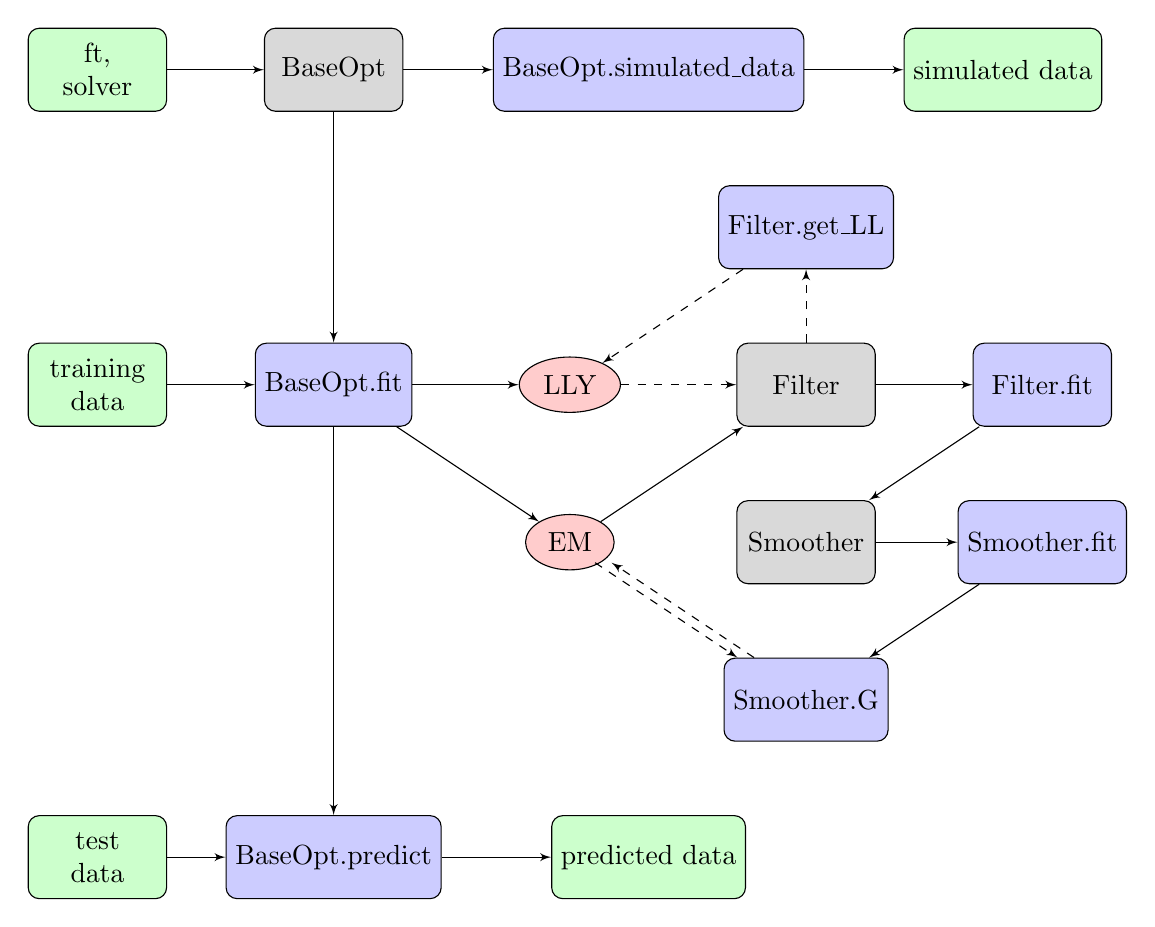
\begin{tikzpicture}[node distance = 2cm, auto]

	% Place nodes
	\node [module] (BaseOpt) {BaseOpt};
	\node [io, left of=BaseOpt, text width = 1cm] (BaseOptInit) {ft, \\ solver};
	\node [method, right of=BaseOpt, node distance=4cm] (simulate) {BaseOpt.simulated\_data};
	\node [io, right of=simulate, node distance=4.5cm] (simdata) {simulated data};
	\node [method, below of=BaseOpt, node distance=4cm] (fit) {BaseOpt.fit};
    \node [algo, right of=fit] (LLY) {LLY};
    \node [algo, below of=LLY, node distance=2cm] (EM) {EM};
    \node [module, right of=LLY] (filter) {Filter};
    \node [method, above of=filter, node distance=2cm] (filterlly) {Filter.get\_LL};
    \node [method, right of=filter, node distance=3cm] (filterfit) {Filter.fit};
    \node [module, below of=filter, node distance=2cm] (smoother) {Smoother};
    \node [method, right of=smoother, node distance=3cm] (smootherfit) {Smoother.fit};
    \node [method, below of=smoother, node distance=2cm] (G) {Smoother.G};
	\node [method, below of=fit, node distance=6cm] (predict) {BaseOpt.predict};
	\node [io, left of=predict, text width = 1cm] (testDf) {test \\ data};
	\node [io, left of=fit, text width = 1.5cm] (trainDf) {training \\ data};
	\node [io, right of=predict, node distance=4cm] (predDf) {predicted data};

	% Draw edges
	\path [line] (BaseOptInit) -- (BaseOpt);
	\path [line] (BaseOpt) -- (simulate);
	\path [line] (simulate) -- (simdata);
	\path [line] (BaseOpt) -- (fit);
	\path [line] (fit) -- (LLY);
	\path [line] (fit) -- (EM);
	\path [line, dashed] (LLY) -- (filter);
	\path [line, dashed] (filter) -- (filterlly);
	\path [line, dashed] (filterlly) -- (LLY);
	\path [line] (EM) -- (filter);
	\path [line] (filter) -- (filterfit);
	\path [line] (filterfit) -- (smoother);
	\path [line] (smoother) -- (smootherfit);
	\path [line] (smootherfit) -- (G);
	\path [line, dashed, transform canvas={xshift=4pt}] (G) -- (EM);
    \path [line, dashed, transform canvas={xshift=-2pt}] (EM) -- (G);
	\path [line] (fit) -- (predict);
	\path [line] (testDf) -- (predict);
	\path [line] (trainDf) -- (fit);
	\path [line] (predict) -- (predDf);
\end{tikzpicture}
    \caption{High level design of \texttt{linkalman}. Green blocks are I/O components, gray blocks are modules, purple blocks are class methods, and red circles are optimizer options. Solid lines indicate the order of model execution. Dotted lines indicate the modules/functions directly involved in numerical optimization.} 
    \label{fig:design}
\end{figure}

The third principle of \texttt{linkalman} is numerical performance. Although \texttt{linkalman} is not designed to be the fastest solver for any specific type of problems, it nevertheless strives to achieve numerical robustness and computational efficiency\footnote{The effort in boosting performance is mostly algorithmic, so there is still ample room for improvement from the programming perspective. For example, the computationally heavy filter updating methods can be written in \texttt{Cython}.}. First of all, I use both Joseph Representation and nearest positive semi-definite matrix technique to ensure positive semi-definiteness of covariance matrices. Secondly, I use sequential filtering and smoothing to further reduce the computational burden from matrix inverse.  

\section{Kalman Filter} \label{sec:filter}
\subsection{Filtering with Known Initial Conditions}
Given a set of measurements over time, and suppose $\theta$ is known. To predict $y_{T+1}$, we need to perform forward filtering. We start by making the following notations:
\begin{align*}
    Y_t &\equiv \{y_1, y_2, ..., y_t\} \\
    X_t &\equiv \{x_1, x_2, ..., x_t\} \\
    \Xi_t &\equiv \{\xi_1,\xi_2,...,\xi_t\} \\
    \hat{\xi}_{t|s} &\equiv E(\xi_t|X_{T},Y_{s};\theta) \\
    P_{t|s} &\equiv E[(\xi_t-\hat{\xi}_{t|s})(\xi_t-\hat{\xi}_{t|s})']
\end{align*}
With the assumption that $w_t$ and $v_t$ are Gaussian white noises, conditional distribution of $y_t$ and $\xi_t$ are fully characterized by Gaussian process with $\hat{\xi}_{t|s}$ and $P_{t|s}$. Now consider at time $t$, we know $Y_t$ and $X_t$, $\hat{\xi}_{t|t-1}$, and $P_{t|t-1}$. By equation (\ref{eq:state_evolve}), we have\footnote{The derivation closely follows Chapter 13 in (\cite{hamilton_1994}). In particular, derivation of equation (\ref{eq:p_tt}) is given in Appendix \ref{ap:iter_proj}.}:
\begin{align}
    \hat{\xi}_{t|t} &= \hat{\xi}_{t|t-1} + K_t(y_t-H_t\hat{\xi}_{t|t-1}-D_tx_t) \label{eq:filter_begin} \\
    K_t &= P_{t|t-1}H_t^{'}\Upsilon_t^{-1} \label{eq:gain} \\
    \Upsilon_t &\equiv H_tP_{t|t-1}H_t^{'} + R_t \\
    P_{t|t} &= P_{t|t-1} - K_tH_tP_{t|t-1} \label{eq:p_tt} \\
    \hat{\xi}_{t+1,t} &= F_t\hat{\xi}_{t|t} + B_tx_t \label{eq:xi_t1} \\
    P_{t+1,t} &= F_tP_{t|t}F_t^{'}+Q_t \label{eq:filter_end}
\end{align}
$K_t$ is the famous Kalman gain matrix. In this subsection, we assume that initial conditions $\hat{\xi}_{1|0}$ and $P_{1|0}$ are known. The Kalman filter proceeds as follows:
\begin{boenumerate}
    \item Given $\theta$, begin with initial value $\hat{\xi}_{1|0}$ and $P_{1|0}$.
    \item Use equation (\ref{eq:filter_begin}) through (\ref{eq:filter_end}) to calculate $\hat{\xi}_{2|1}$, and $P_{2|1}$.
    \item Repeat step 2 for $t\in\{3, 4, ..., T\}$.
\end{boenumerate}

\subsection{Joseph Form and Numerical Robustness}
We define $P_{t|t}$ as a covariance matrix, which is a symmetric positive semi-definite (PSD) matrix, but in practice, we may get $P_{t|t}$ that is neither symmetric nor PSD, due to rounding errors. Look at equation (\ref{eq:p_tt}) again. The subtraction makes calculating $P_{t|t}$ susceptible to rounding errors, sometimes even resulting in negative semi-definite matrix. I use the Joseph form to numerically enforce symmetric PSD. 

The Joseph form (\cite{joseph_1968}) of $P_{t|t}$ is\footnote{For a detailed proof, see Appendix \ref{ap:joseph}}:
\[
    P_{t|t} = [I - K_tH_t]P_{t|t-1}[I - K_tH_t]' + K_tR_tK_t^{'}    
\]
If we guarantee $P_{t|t-1}$ and $R_t$ to be PSD, then $P_{t|t}$ is PSD by construction. Define $M_t$, $L_t$, and $d_t$ as:
\begin{align*}
    M_t &\equiv F_tK_t \\
    L_t &\equiv F_t-M_tH_t \\
    d_t &\equiv y_t - H_t\hat{\xi}_{t|t-1} - D_tx_t
\end{align*}
We are able to obtain a more concise updating rule:
\begin{align}
    \hat{\xi}_{t+1,t} &= F_t\hat{\xi}_{t|t-1} + M_td_t \label{eq:joseph_update_xi} \\
    P_{t+1,t} &= L_tP_{t|t-1}L_t^{'} + M_tR_tM_t^{'} + Q_t \label{eq:joseph_update_P}
\end{align}
Using equation (\ref{eq:joseph_update_xi}) through (\ref{eq:joseph_update_P}) recursively, we may implement Kalman filtering in the Joseph form. 

\subsection{Initialization with Diffuse Filtering} \label{subsec:diff_filter}
So far we have assumed that we know values of $\hat{\xi}_{1|0}$ and $P_{1|0}$. In practice, such information are rarely available. If instead, we know that the time series is stationary, we can use the unconditional mean and variance for $\hat{\xi}_{1|0}$ and $P_{1|0}$. If the time series is at least partially non-stationary, then we should assume no prior information and set $\hat{\xi}_{1|0}=0$ and $P_{1|0}=\infty$ for the non-stationary part of $\xi_t$. A commonly used solution is to set $P_{1|0}$ to some large value (e.g. $\kappa=10^7$) to approximate infinity, but this technique is difficult to implement when the initial condition structure is complex\footnote{See Section 3 of (\cite{doan_2010}) for further discussions.}. Better algorithms exist for exact initialization, and I will discuss one such algorithm that is implemented by \texttt{linkalman}.

Consider $\hat{\xi}_{1|0}$ again. Following (\cite{koopman_1997}), we define $\hat{\xi}_{1|0}$ as:
\begin{align}
    \hat{\xi}_{1|0} = a + A\eta + \Pi\varepsilon \label{eq:init}
\end{align}
$A$ and $\Pi$ are selection matrices, $\eta\sim\mathcal{N}(0,\kappa I)$, and $\varepsilon\sim\mathcal{N}(0,Q_{*})$. Set $0$ for elements in $a$ corresponding to $A$, and stationary means for elements corresponding to $\Pi$. $Q_{*}$ is the ergodic covariance of the stationary component of the model (or process with known initial values). Essentially, equation (\ref{eq:init}) groups $\hat{\xi}_{1|0}$ into two categories. If $\hat{\xi}_{1|0}^i$, the $i$-th element of $\hat{\xi}_{1|0}$, is non-stationary and not known, it has a distribution $\mathcal{N}(0, \kappa)$. With $\kappa\rightarrow\infty$, $\mathcal{N}(0,\kappa)$ captures the fact that we know nothing about the initial value of a non-stationary process\footnote{The specification of equation (\ref{eq:init}), despite its seemingly arbitrariness, is valid, because of the invariance property of diffuse prior. Interested readers can refer to Appendix B of (\cite{doan_2010}) for details.}. If on the other hand, the initial state of $\hat{\xi}_{1|0}^i$ is either known or stationary, It has a proper distribution with unconditional mean and covariances\footnote{If $x_t$ is involved in the state transition process then a process is not stationary unless its transition is not affected by $\{x_t\}_{t\in(-\infty,\infty)}$.}. 

From equation (\ref{eq:init}), we have:
\begin{align}
    \hat{\xi}_{1|0} &= a  \label{eq:init_xi}\\
    P_{1|0} &= \kappa P_{\infty} + P_{*} \label{eq:init_P}
\end{align}
where $P_{\infty}=AA^{'}$ and $P_{*}=\Pi Q_* \Pi^{'}$. By linearity of the filtering process, we can write $P_{t|t-1}$ as:
\begin{align}
    P_{t|t-1} = \kappa P_{\infty,t} + P_{*,t} + \mathcal{O}(\kappa^{-1}) \label{eq:P_diffuse}
\end{align}
where $\mathcal{O}(\kappa^{-1})$ is a function $f(\kappa)<\infty$ as $\kappa\rightarrow\infty$. We can write $\Upsilon_{t}$ as:
\begin{align*}
    \Upsilon_t = \kappa\Upsilon_{\infty,t} + \Upsilon_{*,t} + \mathcal{O}(\kappa^{-1})
\end{align*}
In what follows, I describe the updating rule for exact initialization, for technical details, please refer to Appendix \ref{ap:init_filter}.

Given $\hat{\xi}_{t|t-1}$ and $P_{t|t-1}$, if $\Upsilon_{\infty,t}\neq 0$:
\begin{boenumerate}
    \item Calculate $K_t$ using equation (\ref{eq:K1_diffuse_start}) to (\ref{eq:K1_diffuse_end})
    \item Calculate $\hat{\xi}_{t|t}$ and $P_{t|t}$ from equation (\ref{eq:diff_xi1}) and (\ref{eq:diff_P1})
\end{boenumerate}

If $\Upsilon_{\infty,t}=0$:
\begin{boenumerate}
    \item Calculate $K_t$ using equation (\ref{eq:K2_diffuse})
    \item Calculate $\hat{\xi}_{t|t}$ and $P_{t|t}$ from equation (\ref{eq:diff_xi2}) and (\ref{eq:diff_P2})
\end{boenumerate}

We can update the diffuse Kalman filter with the new expressions for $K_t$, $\hat{\xi}_{t+1,t}$, and $P_{t+1,t}$.

\subsection{Transition to the Usual Kalman Filter}
Diffused initial state is to represent the fact the we have no prior knowledge of initial the state of non-stationary processes. As a result, that state estimate will be dominated by initial data. In other words, the few initial observations are used for form the informative initial conditions, and the rest of the data are used to perform usual Kalman filtering. (\cite{dejong_1991}) and (\cite{durbin_koopman_2003}) show that a diffuse Kalman filter will degenerate to a usual Kalman filter after a few time periods $t_q$, which in general is the number of diffuse initial states. 

A diffuse Kalman filter degenerates to a usual one if $P_{\infty,t}=0$. In practice, we may check if $P_{\infty,t}=0$, but it is subject to numerical errors. (\cite{helske_2016}) implemented a more robust algorithms in his R package \texttt{KFAS}. I provide the procedure below, and interested readers may refer to Appendix \ref{ap:transition} for a simple proof\footnote{For a complete treatment, refer to (\cite{koopman_1997}) for details.}. 

Here I focus on the univariate measurement case, because it is less complex and convertible from multivariate Kalman filters. Define $q_1\equiv rank(P_{\infty,1})$, then by construction of $P_{1,0}$, $q_1$ has rank $q$, where $q$ is the number of diffuse state variables. Let $\varepsilon_t>0$ be some small threshold value\footnote{In practice, I follow (\cite{helske_2016}) and set $\varepsilon_t=\varepsilon\times min(|H_t|;|H_t|>\varepsilon)^2$,  where $\varepsilon=$1e-8 is some base threshold, and $min(|H_t|;|H_t|>\varepsilon)$ is the minimum of the absolute values in $H_t$ that is not $0$.} such that if $\Upsilon_{\infty,t}<\varepsilon_t$, we treat $\Upsilon_{\infty,t}=0$. Define If $\Upsilon_{\infty,t}\geq \varepsilon_t$, then: 
\[
    q_{t+1}=min[q_t-1, rank(P_{\infty,t+1})]
\]

When $q_{t}=0$ for $t=t_q$, the diffuse Kalman filter degenerates into a usual one. This formulation guarantees degeneration to regular Kalman filters.

\subsection{Missing Measurements and Sequential Filtering} \label{subsec:seq_filter}
So far we have assumed that we observe complete measurement $y_t$ for each $t$. If we have incomplete measurements, we can instead update the Kalman Filter sequentially (see (\cite{durbin_koopman_2001}) Section 6.4 and \cite{durbin_koopman_2000} for details), based only on observed measurements. Sequential filtering also boosts speed dramatically in the presence of large measurement dimensions, reducing cost from $\mathcal{O}(n^3)$ to $\mathcal{O}(n)$. In addition, univariate treatment of Kalman filters allows clean formulation with diffuse priors. The techniques developed in this subsection is implemented in \texttt{linkalman} and will be discussed in detail. 

Denote $y_{t:(i)}$ as the $i$-th observed measurement at time $t$, then $y_{t:(1)}$ is the first non-missing univariate measurement at time $t$. Let $(n_t)$ as the index for the last non-missing univatriate measurement at time $t$. Define $\hat{\xi}_{t:(i)}$ and $P_{t:(i)}$ as the state estimates after updating univariate measurement $(i)$ at time $t$:
\begin{align*}
    \hat{\xi}_{t:(i)} &\equiv E(\xi_t|Y_{t-1},y_{t:(1)},...,y_{t:(i-1)},X_T;\theta) \\
    P_{t:(i)} &\equiv Var(\xi_t|Y_{t-1},y_{t:(1)},...,y_{t:(i-1)},X_T;\theta) 
\end{align*}

In addition, at the beginning of time $t$ before any Kalman updating, we have:
\begin{align}
    \hat{\xi}_{t:(1)} &\equiv E(\xi_{t}|Y_{t-1};\theta)\nonumber \\
    &= F_{t-1}\hat{\xi}_{t-1:(n_{t-1}+1)|t-1:(n_{t-1})}+B_{t-1}x_{t-1} \label{eq:diff_xi_seq0} \\
    P_{t:(1)} &\equiv Var(\xi_{t}|Y_{t-1};\theta) \nonumber \\
    &= F_{t-1}P_{t-1:(n_{t-1}+1)|t-1:(n_{t-1})}F_{t-1} + Q_{t-1} \label{eq:diff_P_seq0}
\end{align}

For sequential filtering to work, we need $R_t$ to be diagonal. In the case where $R_t$ is not diagonal, we can use LDL Decomposition\footnote{In practice, I perform LDL Decomposition with \texttt{scipy.linalg.ldl}.} to transform the original BSTS model into one with independent measurement noise. Given that $R_t$ is PSD, we have $R_t = l_t\Lambda_tl_t^{'}$. Pre-multiply equation (\ref{eq:measure}) by $l_t^{-1}$, and we have\footnote{Due to special properties of triangular matrices, in practice, I perform matrix inverse on triangular matrix with \texttt{scipy.linalg.lapack.dtrtri} subroutine.}:
\begin{align}
    \tilde{y}_t = \tilde{H}_t\xi_{t} + \tilde{D}_{t}x_t + \tilde{w}_t \label{eq:ldl}
\end{align}
where $\tilde{(\cdot)}_t = l_t^{-1}(\cdot)_t$. In the following sections, I will omit the $(\sim)$ sign, and assume $R_t$ is always diagonal.

For a BSTS model with diagonal $R_t$, equation (\ref{eq:measure}) then becomes:
\begin{align*}
    y_t &= 
    \begin{pmatrix}
        y_{t:(1)} \\
        \vdots \\ 
        y_{t:(n_t)}
    \end{pmatrix} 
    = \begin{pmatrix}
        H_{t:(1)}\xi_t + D_{t:(1)}x_t + w_{t:(1)} \\
        \vdots \\
        H_{t:(n_t)}\xi_t + D_{t:n_t}x_t + w_{t:(n_t)}
    \end{pmatrix}
\end{align*}
where $H_{t:(i)}$ and $D_{t:(i)}$ are the $(i)$-th row of $H_t$ and $D_t$. 

We initialize the measurement update process with $\hat{\xi}_{1:(1)}$ and $P_{1:(1)}$ from equation (\ref{eq:init_xi}) and (\ref{eq:init_P}). Define $\Upsilon_{t:(i)}$ as:
\begin{align*}
    \Upsilon_{t:(i)} = H_{t:(i)}P_{t:(i)}H_{t:(i)}^{'} + R_{t:(i)}
\end{align*}
where $R_{t:(i)}$ is the $(i)$-th diagonal value of $R_{t}$. For $\Upsilon_{t:(i)}$, we have:
\begin{align*}
    \Upsilon_{\infty, t:(i)} &= H_{t:(i)}P_{\infty, t:(i)}H_{t:(i)}^{'} \\
    \Upsilon_{*,t:(i)} &= H_{t:(i)}P_{*,t:(i)}H_{t:(i)}^{'} + R_{t:(i)}
\end{align*}

For each successive measurement $(i)$, if $\Upsilon_{\infty,t:(i)}\neq0$, we have:
\begin{align}
    \hat{\xi}_{t:(i+1)} = & \hat{\xi}_{t:(i)} + K_{t:(i)}^{(0)}d_{t:(i)} + \mathcal{O}(\kappa^{-1}) \label{eq:diff_seq_xi1} \\
    P_{t:(i+1)} =& \kappa(I-K_{t:(i)}^{(0)}H_{t:(i)})P_{\infty,t:(i)}(I-K_{t:(i)}^{(0)}H_{t:(i)})^{'} \label{eq:diff_seq_P1} \\
        & + (I-K_{t:(i)}^{(0)}H_{t:(i)})P_{*,t:(i)}(I-K_{t:(i)}^{(0)}H_{t:(i)})^{'} \nonumber \\
        & + K_{t:(i)}^{(0)}R_{t:(i)}K_{t:(i)}^{(0)'} + \mathcal{O}(\kappa^{-1}) \nonumber
\end{align}
where
\begin{align*}
    d_{t:(i)} &= y_{t:(i)} - H_{t:(i)}\hat{\xi}_{t:(i)}-D_{t:(i)}x_t \\
    K_{t:(i)}^{(0)} &= \frac{P_{\infty,t:(i)}H_{t:(i)}^{'}}{\Upsilon_{\infty,t:(i)}} 
        =\frac{P_{\infty,t:(i)}H_{t:(i)}^{'}}{H_{t:(i)}P_{\infty, t:(i)}H_{t:(i)}^{'}}
\end{align*}

If $\Upsilon_{\infty,t:(i)}=0$ and $P_{\infty,t:(i-1)}\neq 0$, we have:
\begin{align}
    \hat{\xi}_{t:(i+1)} =& \hat{\xi}_{t:(i)} + K_{t:(i)}^{(*)}d_{t:(i)} + \mathcal{O}(\kappa^{-1}) \label{eq:diff_seq_xi0} \\
    P_{t:(i+1)} =& \kappa P_{\infty,t:(i)} + (I-K_{t:(i)}^{(*)}H_{t:(i)})P_{*,t:(i)}(I-K_{t:(i)}^{(*)}H_{t:(i)})^{'} \label{eq:diff_seq_P0} \\
        &+ K_{t:(i)}^{(*)}R_{t:(i)}K_{t:(i)}^{(*)'} + \mathcal{O}(\kappa^{-1}) \nonumber 
\end{align}
where
\begin{align*}
    K_{t:(i)}^{(*)} &= \frac{P_{*,t:(i)}H_{t:(i)}^{'}}{\Upsilon_{*,t:(i)}} = \frac{P_{*,t:(i)}H_{t:(i)}^{'}}{H_{t:(i)}P_{*,t:(i)}H_{t:(i)}^{'} + R_{t:(i)}}
\end{align*}

If $\Upsilon_{\infty,t:(i)}=0$ and $P_{\infty,t:(i-1)}=0$, the diffuse Kalman filter degenerates into a usual one, and instead of using equation (\ref{eq:diff_seq_P0}), we use:
\begin{align}
    P_{t:(i+1)} =& (I-K_{t:(i)}^{(*)}H_{t:(i)})P_{*,t:(i)}(I-K_{t:(i)}^{(*)}H_{t:(i)})^{'} + K_{t:(i)}^{(*)}R_{t:(i)}K_{t:(i)}^{(*)'} \label{eq:usual_seq_P0} 
\end{align}

Now we may proceed with sequential filtering as follows:
\begin{boenumerate}
    \item Initialize state conditions using equation (\ref{eq:init_xi}) and (\ref{eq:init_P}) 
    \item For period $t$, calculate $\hat{\xi}_{t:(0)}$ and $P_{t:{(0)}}$ using equation (\ref{eq:diff_xi_seq0}) and (\ref{eq:diff_P_seq0}) \label{step:seq_filter_begin}
    \item Use LDL transformation to obtain diagonalized measurement equation (\ref{eq:ldl})
    \item If $\Upsilon_{\infty,t:(i)}\neq0$, use equation (\ref{eq:diff_seq_xi1}) and (\ref{eq:diff_seq_P1}) to update $\hat{\xi}_{t:(i+1)}$ and $P_{t:(i+1)}$
    \item If $\Upsilon_{\infty,t:(i)}=0$ and $\hat{q}_{t:(i)}>0$, use equation (\ref{eq:diff_seq_xi0}) and (\ref{eq:diff_seq_P0}) to update $\hat{\xi}_{t:(i+1)}$ and $P_{t:(i+1)}$ 
    \item If $\hat{q}_{t:(i)}=0$, use equation (\ref{eq:diff_seq_xi0}) and (\ref{eq:usual_seq_P0}) to update $\hat{\xi}_{t:(i+1)}$ and $P_{t:(i+1)}$ 
    \item Update $\hat{q}_{t:(i+1)} = min[\hat{q}_{t:(i)}-1, q_{t:(i+1)}]$. If $i=n_t$, $\hat{q}_{t+1:(1)}=\hat{q}_{t:(n_t+1)}$ \label{step:seq_filter_end}
    \item Repeat step (\ref{step:seq_filter_begin}) through (\ref{step:seq_filter_end}) for $t\in\{1,2,...,T\}$
\end{boenumerate}

An alternative view of the procedure is to treat $y_t$ as $(y_{t:(1)},...,y_{t:(n_t)})$, with $F_{t:(i)}=I$, $Q_{t:(i)}=0$, and $B_{t:(i)}=0$ for $i\in{1,...,n_t}$. The transition from $[t:(n_t)]$ to $[t+1:(1)]$ with transition matrices $F_t$, $Q_t$, and $B_t$ is broken down into two steps: $[t:(n_t)]$ to $[t:(n_t+1)]$ with $F_{t:(n_t)}=I$, $Q_{t:(n_t)}=0$, and $B_{t:(n_t)}=0$, then $[t:(n_t+1)]$ to $[t+1:(1)]$ with $F_{t:(n_t+1)}=F_t$, $Q_{t:(n_t+1)}=Q_t$, and $B_{t:(n_t+1)}=B_t$. Note that the second step does not involve measurement update.

\section{Kalman Smoother} \label{sec:smoother}
\subsection{State Smoother}
In Section \ref{sec:filter}, we use Kalman Filter to find $\{\hat{\xi}_{t|t}, K_t, P_{t|t}, \hat{\xi}_{t|t-1}, P_{t|t-1}\}$ for each $t$. If a dataset is given, we have the entire measurement sequence $Y_T$. Kalman Smoother is a technique of integrating information up to $T$ to infer $\xi_t$ at time $t$, $\hat{\xi}_{t|T}$ and $P_{t|T}$. 

Suppose in addition to state estimates from Kalman Filter, we also want to know $\hat{\xi}_{t|T}$ and $P_{t|T}$. The technique for computing $\hat{\xi}_{t|T}$ and $P_{t|T}$ is called backwards smoothing\footnote{See (\cite{dejong_1989}) for details. I also provided a proof in Appendix \ref{ap:smooth} that is consistent with notations in this document and has more details.}. Here I present the iterative formula for Kalman smoothing. Following derivations in Appendix \ref{ap:smooth}, I define two auxiliary variables: $r_{t}$ and $N_{t}$, where $r_T=0$, $N_T=0$, and:
\begin{align}
    r_{t-1} &= H_t^{'}\Upsilon_t^{-1}d_t + L_t^{'}r_t \label{eq:r1t} \\
    N_{t-1} &= H_t^{'}\Upsilon_t^{-1}H_t + L_t^{'}N_tL_t \label{eq:N1t}
\end{align}

Using $\{r_t\}_{1,...,T}$ and $\{N_t\}_{1,...,T}$, we have the iterative formulation for $\hat{\xi}_{t|T}$ and $P_{t|T}$:
\begin{align}
    \hat{\xi}_{t|T} &= \hat{\xi}_{t|t-1} + P_{t|t-1}r_{t-1} \label{eq:smooth_state2} \\
    P_{t|T} &= P_{t|t-1}- P_{t|t-1}N_{t-1}P_{t|t-1} \label{eq:smooth_P2}
\end{align}

As we will see in Section \ref{subsec:EM} and Appendix \ref{ap:log}, we also need to calculate covariance matrices of smoothed estimators. Define $P_{t,s|n}$ as:
\begin{align*}
    P_{t,s|n}\equiv Cov(\xi_t,\xi_{s}|Y_n,X_T;\theta)
\end{align*}

Following (\cite{koopman_1992}), (\cite{dejong_1988}), and (\cite{dejong_1989})\footnote{See Appendix \ref{ap:cov_smooth} for details.}, we have for $1\leq t < j \leq T$:
\begin{align*}
    P_{t,j|T} = P_{t|t-1}\prod_{i=t}^{j-1}L_i^{'}(I-N_{j-1}P_{j|j-1}) 
\end{align*}

In particular, we are interested in:
\begin{align}
    P_{t,t+1|T} = P_{t+1,t|T}^{'} = P_{t|t-1}L_t^{'}(I-N_tP_{t+1|t}) \label{eq:cov_smooth}
\end{align}

To perform backwards smoothing, we can simply start at time $T$ with $r_T=0$ and $N_T=0$, then use equation (\ref{eq:r1t}) through (\ref{eq:cov_smooth}) for $t\in\{T-1,T-2,...,1\}$ to obtain $\{\hat{\xi}_{t|T}\}_{1,2,...,T}$, $\{P_{t|T}\}_{1,2,...,T}$ and $\{P_{t,t+1|T}\}_{1,2,...,T}$.

\subsection{Rounding Errors and Nearest PSD}
Note that for Kalman Smoother, we don't have Joseph Form formulation, and therefore we may still get non-PSD covariance matrix and cause the smoother to fail. By construction, I guarantee symmetry of covariance matrices. Therefore, we may check PSD using Cholesky Decomposition, which is efficient under symmetry conditions.

If a covariance matrix $C$ is not PSD, we can use the nearest PSD matrix with the techniques developed by (\cite{higham_1988}). Omitting technical details, it amounts to replacing $C$ with $\bar{C}$, where $\bar{A}$ is be calculated as:
\begin{align*}
    C &= USV^{'} \\
    \Sigma &= VSV^{'} \\
    \bar{C} &= \frac{\Sigma + \Sigma^{'} + C + C^{'}}{4}
\end{align*}
where the first equality is the SVD decomposition of $C$. By construction, $N_{t-1}$ is PSD, then we only need to correct $P_{t|T}$ if necessary. 

\subsection{Diffuse Smoother}
When initial conditions are unknown, we can use diffuse smoothers. Similar to diffuse filters, we expand $P_{t|T}$, $r_{t-1}$, and $N_{t-1}$. Appendix \ref{ap:init_smoother} provide detailed derivation of recursive formula, so here I will just give the result. First of all, I give the expression for $\hat{\xi}_{t|T}$, $P_{t|T}$, and $P_{t,t+1|T}$ as:
\begin{align}
    \hat{\xi}_{t|T} =& \hat{\xi}_{t|t-1} + P_{*,t}r_{t-1}^{(0)}+P_{\infty,t}r_{t-1}^{(1)}+\mathcal{O}(\kappa^{-1}) \label{eq:diff_xi} \\
    P_{t|T} =& P_{*,t} - \langle P_{\infty,t}N_{t-1}^{(1)}P_{*,t}\rangle - P_{*,t}N_{t-1}^{(0)}P_{*,t} 
        - P_{\infty,t}N_{t-1}^{(2)}P_{\infty,t} + \mathcal{O}(\kappa^{-1}) \label{eq:diff_P} \\
    P_{t,t+1|T} =& (P_{*,t}L_t^{(0)'}+P_{\infty,t}L_t^{(1)'})(I-N_t^{(1)}P_{\infty,t+1}-N_t^{(0)}P_{*,t+1}) \nonumber \\
    &- P_{\infty,t}L_t^{(0)'}(N_t^{(2)}P_{\infty,t+1}+N_t^{(1)}P_{*,t+1}) + \mathcal{O}(\kappa^{-1}) \label{eq:diff_Pcov}
\end{align}

Now we need to compute $r_{t-1}$, and $N_{t-1}$. If $\Upsilon_{\infty,t}\neq 0$, we use:
\begin{boenumerate}
    \item Begin with $r_{t_q}^{(0)}=r_{t_q}$, $r_{t_q}^{(1)}=0$, $N_{t_q}^{(0)}=N_{t_q}$, and $N_{t_q}^{(1)}=N_{t_q}^{(2)}=0$
    \item Use equation (\ref{eq:r_inf_start}) through (\ref{eq:r_inf_end}) to compute expansions of $r_{t-1}$
    \item Use equation (\ref{eq:N_inf_start}) through (\ref{eq:N_inf_end}) to compute expansions of $N_{t-1}$
\end{boenumerate}

If $\Upsilon_{\infty,t}=0$, we instead use\footnote{Note that we do not have to provide initial values in this case, as diffuse filters always end with $\Upsilon_{\infty,t}\neq 0$.}:
\begin{boenumerate}
    \item Use equation (\ref{eq:r_0_start}) through (\ref{eq:r_0_end}) to compute expansions of $r_{t-1}$
    \item Use equation (\ref{eq:N_0_start}) through (\ref{eq:N_0_end}) to compute expansions of $N_{t-1}$
\end{boenumerate}

We can then calculate $\hat{\xi}_{t|T}$, $P_{t|T}$, and $P_{t,t+1|T}$ through equation (\ref{eq:diff_xi}) through (\ref{eq:diff_Pcov}). 

\subsection{Sequential Smoother}
As with the case of Kalman filtering, calculating $\Upsilon_t^{-1}$ is expensive and subject to failure due to rounding errors. (\cite{durbin_koopman_2000}) proposes sequential smoothing to greatly improved the efficiency and robustness of Kalman Smoothers. The univariate approach in Kalman filter essentially treats observations flowing in one at a time, so we can readily adapt our smoother.

Define $y_{t:(i)}$ as the $i$-th non-missing measurement of $y_t$. To derive the univariate formula for diffuse smoothers, we can treat smoothing between two observations within the same period as if the transition matrix is $F_{t-1}$ between $t-1:(n_t)$ and $t:(1)$, and is an identity matrix if otherwise. In addition, for notational purpose, we can add $r_{t:(0)}$ and $N_{t:(0)}$. It is easy to see $r_{t:(0)}=r_t$, and $N_{t:(0)}=N_t$. For the case $(i)\leq(n_t)$, if $\Upsilon_{\infty,t:(i)}\neq0$, the recursive formula for $r_{t-1}$ and $N_{t-1}$ are:
\begin{align}
    r_{t:(i-1)}^{(0)} =& L_{t:(i)}^{(0)'}r_{t:(i)}^{(0)} \label{eq:diff_uni_start} \\
    r_{t:(i-1)}^{(1)} =& H_{t:(i)}^{'}\left(\frac{d_{t:(i)}}{\Upsilon_{\infty,t:(i)}}-K_{t:(i)}^{(1)'}r_{t:(i)}^{(0)}\right)+L_{t:(i)}^{(0)'}r_{t:(i)}^{(1)} \nonumber \\
    =& \frac{H_{t:(i)}^{'}d_{t:(i)}}{\Upsilon_{\infty,t:(i)}} + L_{t:(i)}^{(1)'}r_{t:(i)}^{(0)} + L_{t:(i)}^{(0)'}r_{t:(i)}^{(1)} \\
    N_{t:(i-1)}^{(0)} =& L_{t:(i)}^{(0)'}N_{t:(i)}^{(0)}L_{t:(i)}^{(0)} \\
    N_{t:(i-1)}^{(1)} =& \frac{H_{t:(i)}^{'}H_{t:(i)}}{\Upsilon_{\infty,t:(i)}} + \langle L_{t:(i)}^{(1)'}N_{t:(i)}^{(0)}L_{t:(i)}^{(0)}\rangle + L_{t:(i)}^{(0)'}N_{t:(i)}^{(1)}L_{t:(i)}^{(0)} \\
    N_{t:(i-1)}^{(2)} =& -\frac{H_{t:(i)}^{'}H_{t:(i)}\Upsilon_{*,t:(i)}}{\Upsilon_{\infty,t:(i)}^{2}} + \langle L_{t:(i)}^{(1)'}N_{t:(i)}^{(1)}L_{t:(i)}^{(0)}\rangle \nonumber \\
    &+L_{t:(i)}^{(0)'}N_{t:(i)}^{(2)}L_{t:(i)}^{(0)} + L_{t:(i)}^{(1)'}N_{t:(i)}^{(0)}L_{t:(i)}^{(1)} \\
    L_{t:(i)}^{(0)} =& I-K_{t:(i)}^{(0)}H_{t:(i)}= I-\frac{P_{\infty,t:(i)}H_{t:(i)}^{'}H_{t:(i)}}{H_{t:(i)}P_{\infty,t:(i)}H_{t:(i)}^{'}} \\
    L_{t:(i)}^{(1)} =& - K_{t:(i)}^{(1)}H_{t:(i)}=-\frac{(P_{*,t:(i)}H_{t:(i)}^{'}-K_{t:(i)}^{(0)}\Upsilon_{*,t:(i)})H_{t:(t)}}{H_{t:(i)}P_{\infty,t:(i)}H_{t:(i)}^{'}}
\end{align}

Similarly, if $\Upsilon_{\infty,t:(i)}=0$ and $t<t_q$, the recursive formula for $r_{t:(i)}$ and $N_{t:(i)}$ are:
\begin{align}
    r_{t:(i-1)}^{(0)} &= \frac{H_{t:(i)}^{'}d_{t:(i)}}{H_{t:(i)}P_{*,t:(i)}H_{t:(i)}^{'}+R_{t:(i)}} + (I-K_{t:(i)}^{(*)}H_{t:(i)})^{'}r_{t:(i)}^{(0)} \nonumber \\
    &= \frac{H_{t:(i)}^{'}d_{t:(i)}}{\Upsilon_{*,t:(i)}} + L_{t:(i)}^{(*)'}r_{t:(i)}^{(0)} \\
    r_{t:(i-1)}^{(1)} &= r_{t:(i)}^{(1)} \\ 
    N_{t:(i-1)}^{(0)} &= \frac{H_{t:(i)}^{'}H_{t:(i)}}{H_{t:(i)}P_{*,t:(i)}H_{t:(i)}^{'}+R_{t:(i)}}+(I-K_{t:(i)}^{(*)}H_{t:(i)})^{'}N_{t:(i)}^{(0)}(I-K_{t:(i)}^{(*)}H_{t:(i)}) \nonumber \\
    &= \frac{H_{t:(i)}^{'}H_{t:(i)}}{\Upsilon_{*,t:(i)}} + L_{t:(i)}^{(*)'}N_{t:(i)}^{(0)}L_{t:(i)}^{(*)} \\
    N_{t:(i-1)}^{(1)} &= (I-K_{t:(i)}^{(*)}H_{t:(i)})^{'}N_{t:(i)}^{(1)}(I-K_{t:(i)}^{(*)}H_{t:(i)}) \nonumber \\
    &= L_{t:(i)}^{(*)'}N_{t:(i)}^{(1)}L_{t:(i)}^{(*)} \\
    N_{t:(i-1)}^{(2)} &= N_{t:(i)}^{(2)} \\
    K_{t:(i)}^{(*)} &= \frac{P_{*,t:(i)}H_{t:(i)}^{'}}{H_{t:(i)}P_{*,t:(i)}H_{t:(i)}^{'}+R_{t:(i)}} \\
    L_{t:(i)}^{(*)} &= I - K_{t:(i)}^{(*)}H_{t:(i)}
\end{align}

For the regular Kalman smoother where $t\geq t_q$, the formula are: 
\begin{align}
    r_{t:(i-1)}^{(0)} &= \frac{H_{t:(i)}^{'}d_{t:(i)}}{\Upsilon_{*,t:(i)}} + L_{t:(i)}^{(*)'}r_{t:(i)}^{(0)} \\
    N_{t:(i-1)}^{(0)} &= \frac{H_{t:(i)}^{'}H_{t:(i)}}{\Upsilon_{*,t:(i)}} + L_{t:(i)}^{(*)'}N_{t:(i)}^{(0)}L_{t:(i)}^{(*)} 
\end{align}

Essentially, we only update $r_{t:(i-1)}^{(0)}$ and $N_{t:(i-1)}^{(0)}$. 

For the case $(i)=(0)$, then the recursive formula for $r_{t-1:(n_{t-1})}$ and $N_{t-1:(n_{t-1})}$ become:
\begin{align}
    r_{t-1:(n_{t-1})}^{(0)} &= F_{t-1}^{'}r_{t:(0)}^{(0)} \\
    r_{t-1:(n_{t-1})}^{(1)} &= F_{t-1}^{'}r_{t:(0)}^{(1)} \\
    N_{t-1:(n_{t-1})}^{(0)} &= F_{t-1}^{'}N_{t:(0)}^{(0)}F_{t-1} \\
    N_{t-1:(n_{t-1})}^{(1)} &= F_{t-1}^{'}N_{t:(0)}^{(1)}F_{t-1} \\
    N_{t-1:(n_{t-1})}^{(2)} &= F_{t-1}^{'}N_{t:(0)}^{(2)}F_{t-1} \label{eq:diff_uni_end}
\end{align}

Now we can find the univariate versions of $\hat{\xi}_{t|T}$, $P_{t|T}$, and $P_{t,t+1|T}$ by applying equation (\ref{eq:diff_uni_start}) through (\ref{eq:diff_uni_end}) to equation (\ref{eq:diff_xi}) through (\ref{eq:diff_Pcov}). In particular, in the case of univariate smoother, $\hat{\xi}_{t:(i)}=\hat{\xi}_{t:(1)}$ and $P_{t:(i)}=P_{t:(1)}$, because there is no change in $t$\footnote{It is easy to show the equivalence by expanding the expression of $\hat{\xi}_{t|T}^{(i+1)}$ and comparing it against $\hat{\xi}_{t|T}^{(i)}$.}. In addition, EM algorithm requires computing $P_{t,t+1|T}$ even if $t$ or $t+1$ has fully missing measurements. Unlike Kalman filters, we only need to store one set of state values for each $t$. Define $P_{t,t+1|T} \equiv P_{t:(n_t+1),t+1:(1)|T}$. If $t<t_q$, we have:
\begin{align}
    \hat{\xi}_{t:(1)|T} =& \hat{\xi}_{t:(1)} + P_{*,t:(1)}r_{t:(0)}^{(0)} + P_{\infty,t:(1)}r_{t:(0)}^{(1)} \label{eq:diff_smooth_start} \\
    P_{t:(1)|T} =& P_{*,t:(1)} - \langle P_{\infty,t:(1)}N_{t:(0)}^{(1)}P_{*,t:(1)} \rangle - P_{*,t:(1)}N_{t:(0)}^{(0)}P_{*,t:(1)} \nonumber \\
        &- P_{\infty,t:(1)}N_{t:(0)}^{(2)}P_{\infty,t:(1)} \\
    P_{t,t+1|T} =& P_{*,t:(n_t+1)}F_t^{'}(I-N_{t+1:(0)}^{(1)}P_{\infty,t+1:(1)} - N_{t+1:(0)}^{(0)}P_{*,t+1:(1)}) \nonumber \\
    &- P_{\infty,t:(n_t+1)}F_t^{'}(N_{t+1:(0)}^{(2)}P_{\infty,t+1:(1)}+N_{t+1:(0)}^{(1)}P_{*,t+1:(1)})
\end{align}

If $t \geq t_q$, we have:
\begin{align}
    \hat{\xi}_{t:(1)|T} &= \hat{\xi}_{t:(1)} + P_{t:(1)}r_{t:(0)} \\
    P_{t:(1)|T} &= P_{t:(1)} - P_{t:(1)}N_{t:(0)}P_{t:(1)} \\
    P_{t,t+1|T} &= P_{t:(n_t+1)}F_t^{'}(I - N_{t+1:(0)}P_{t+1:(1)}) \label{eq:diff_smooth_end}
\end{align}

Recall that the state estimates are the same between $t:(i)$ and $t:(i+1)$ for any given time, so we may choose any measurement index $(i)$. Equation (\ref{eq:diff_smooth_start}) and (\ref{eq:diff_smooth_end}) are preferred here because their indexing are consistent with those in Kalman filters and smoothers, and are capable of handling fully missing measurements.

\subsection{Interpolating Missing Measurements}
Quite often we would like to know the smoothed value of missing measurements (e.g. counterfactuals for studying treatment effects), this subsection provides formula for smoothed means and variances of $y_t$ (interested readers may refer to Appendix \ref{ap:interp} for details):
\begin{align}
    E(y_t^{(1)}|Y_t^{(1)}) &= y_t^{(1)} \label{eq:smoothed_y1_mean} \\
    Var(y_t^{(1)}|Y_t^{(1)}) &= 0 \\
    E(y_t^{(2)}|Y_t^{(1)}) &= H_t^{(2)}\hat{\xi}_{t|T} + D_t^{(2)}x_t + \mathcal{B}_t\epsilon_t \label{eq:smoothed_y2_mean} \\
    Var(y_t^{(2)}|Y_t^{(1)}) &= R_t^{(2, 2)} - R_t^{(2, 1)}\left(R_t^{(1, 1)}\right)^{-1}R_t^{(1, 2)} + 
        \left(H_t^{(2)}-\mathcal{B}_tH_t^{(1)}\right)P_{t|T}\left(H_t^{(2)}-\mathcal{B}_tH_t^{(1)}\right)^{'} \label{eq:smoothed_y2_cov}
\end{align}

Using equation (\ref{eq:smoothed_y1_mean}) through (\ref{eq:smoothed_y2_cov}). We have the smoothed distribution of missing measurements. Note that in practice, I restore the index of smoothed estimates of $y_t$ to their original order. It is also worth noting that when all measurements at time $t$ are missing, equation (\ref{eq:smoothed_y2_mean}) and (\ref{eq:smoothed_y2_cov}) becomes:
\begin{align*}
    E(y_t^{(2)}|Y_t^{(1)}) &= H_t\hat{\xi}_{t|T} + D_tx_t \\
    Var(y_t^{(2)}|Y_t^{(1)}) &= R_t + H_tP_{t|T}H_t^{'} 
\end{align*}

\section{Parameter Estimation} \label{sec:param}
Up to this point, we have assumed that system matrices of a BSTS model is known. In practice, such conditions are rarely met. In this section, I will present two methods: numerical maximization and EM algorithm. Direct numerical maximization has the advantage of faster convergence close to true values, and it does not requires Kalman smoothers, which requires vast computational costs. On the other hand, the EM algorithm converges faster at the beginning, and has a cleaner derivation. It is important to note, however, that the two approaches are consistent, but not unbiased. Therefore, users should practice with caution when using likelihood based models for parameter estimation. In what follows, I provide more details about the two algorithms in the case of diffuse priors.

\subsection{Initialization with Lyapunov Equation and Directed Graphs} 
If we are dealing with a BSTS model with constant system matrices, and $P_{1|0}$ or $\hat{\xi}_{1|0}$ is not provided, it is possible to compute them\footnote{For BSTS models with time varying system matrices, it is advised to supply user-defined $\hat{\xi}_{1|0}$ and $P_{1|0}$.}. Effectively we want to find the ergodic mean and variance (or their diffuse counterparts). First consider $P_{1|0}$. To find ergodic variance is equivalent to solving a Lyapunov stability equation:
\begin{align}
    FP_{1|0}F^{'} + Q = P_{1|0} \label{eq:lyap}
\end{align}
where $F$ is $F_t$ without the time subscript $t$. I use \texttt{scipy.linalg.solve\_discrete\_lyapunov} function to find $P_{1|0}$. If there is at least one unit root for $F$, the resulting $P_{1|0}$ will have very large values along the diagonal axis at indices that we may treat as diffuse states. $Q$ is the assumed to be common error covariance matrix for state transition errors up to$t=0$\footnote{If $Q_t$ or any system matrix related to state transitioning is not constant or unknown, we should use diffuse initialization for these states.}. It is important to keep $Q$ a positive semi-definite\footnote{There are several techniques to ensure both uniqueness and unboundedness in parametrizing $Q$. \texttt{linkalman} uses the Cholesky decomposition technique described in (\cite{pinheiro1996unconstrained}), which also outlines several alternative approaches.}, or we have pathological systems. 

In addition, we may run into BSTS models with explosive roots (i.e. eigenvalues of $F$ are greater than one), equation (\ref{eq:lyap}) still generate a finite (but unstable) $P_{1|0}$ and fails to detect the diffuse state. In such cases, I use techniques in graph theory and first partition $F$ into several strongly connected components\footnote{I use the \texttt{networkx} package to find such components.}. I then calculate the largest eigenvalue in each component, and label these states as diffuse by setting a very large value on the corresponding diagonal values of $F$. Now the explosive states are properly marked, so solving a Lyapunov Equation will produce the correction partition between the diffuse component and the ergodic component of $P_{1|0}$. Note, however, that the assumption of marginal likelihood correction may be violated\footnote{See (\cite{francke_etal_2010}) for details.}. It is advised that users provide sensible estimates for the initial state.

The solution for $\hat{\xi}_{1|0}$ is easier to obtain. Consider the following:
\begin{align*}
    \hat{\xi}_{1|0} &= F\hat{\xi}_{1|0} + Bx \\
    &= (I - F)^{-1}Bx
\end{align*}
where $B$ and $x$ are $B_t$ and $x_t$ without $t$, respectively. In practice, it is easier to set to $0$ the rows of $B$, and $F$ corresponding to the diffuse states. Alternatively, users may provide precomputed or customized $P_{1|0}$ and $\hat{\xi}_{1|0}$. It is also very important to conduct sanity checks on system matrices to avoid pathological systems (e.g. $\xi_{t} = \xi_t + v_t$).

\subsection{Numerical Maximization} \label{subsec:NM}
This section follows closely (\cite{durbin_koopman_2001}) with marginal likelihood corrections from (\cite{francke2010likelihood}) and (\cite{harville1974bayesian}). First we parameterize system matrices. To ensure PSD of $Q_t$ and $R_t$ while allowing unconstrained parameterization, I use Cholesky decomposition described in (\cite{pinheiro1996unconstrained}). Next, I provide the expression for marginal likelihood\footnote{Interested readers may refer to Appendix \ref{ap:NL}.} $l_m(Y_T)$ as:
\begin{align}
    l_m(Y_T) =& Const - \frac{1}{2}\sum_{t=1}^{t_q-1}\sum_{i=1}^{n_t}\Psi_{t:(i)} - \frac{1}{2}\sum_{t=t_q}^{T}\sum_{i=1}^{n_t}\left(log|\Upsilon_{t:(i)}| + \frac{d_{t:(i)}^{'}d_{t:(i)}}{\Upsilon_{t:(i)}}\right) + \frac{1}{2}log\left| \sum_{t=1}^{T}(Z_t^{'}Z_t) \right| \label{eq:NM_likelihood} \\
    \Psi_{t:(i)} =& \begin{cases}
        log|\Upsilon_{\infty,t:(i)}| & \Upsilon_{\infty,t:(i)} > 0 \\
        log|\Upsilon_{*,t:(i)}| + \frac{d_{t:(i)}^{'}d_{t:(i)}}{\Upsilon_{*,t:(i)}} & \Upsilon_{\infty,t:(i)}=0
    \end{cases} \nonumber \\
    Z_t &= H_t\phi_t \label{eq:marginal_correct} \\
    \phi_{t+1} &= F_t\phi_t \nonumber \\
    \phi_1 &= A \nonumber
\end{align}

Note that equation (\ref{eq:NM_likelihood}) only requires Kalman filters, so it avoids costly Kalman smoothers and is faster to evaluate. In the univariate case, $H_t$ is $\tilde{H}_t$, and if the $i$-th measurement is missing, the $i$-th row of $H_t$ is $0$.  In practice, we can use popular numerical optimization packages such as \texttt{scipy} and \texttt{nlopt} to solve it numerically.

\subsection{EM Algorithm} \label{subsec:EM}
One disadvantage of numerical maximization is the speed of the convergence is slow at the beginning. In addition, we need to run the Kalman filter for every parameter evaluation. As an alternative, EM algorithm proposed by (\cite{shumway_stoffer_1982}) has a better early-stage performance\footnote{Given that the intended purpose of \texttt{linkalman} is solving BSTS models with sophisticated model structures, I use non-gradient-based methods. As a result, the primary advantage of EM algorithm (i.e. ease to compute derivatives) is not utilized, and the performance of EM algorithm is inferior to numerical methods.}. The EM algorithm converges to a local optimum iteratively, and in particular, within each iteration, the Kalman smoother is evaluated only once. Its rate of convergence is substantially slower than numerical optimization in the neighborhood of the true parameters. One may use EM algorithm to cold start the optimization, then switch to numerical optimization to fine-tune the estimates. Note that equations used by EM algorithms are closely related to score functions, which can be used by gradient-based algorithms for fast optimization. In what follows, I will provide details of implementing the EM algorithm\footnote{For technical details, refer to Appendix \ref{ap:EM_proof}.}.  

The log likelihood function for a BSTS model is:
\begin{align*}
    L(Y_T|X_T; \theta) &= log[\mathbb{P}(Y_T|X_T;\theta)]
\end{align*}

Following equation (\ref{eq:Q}), we maximize marginal $L(Y_T|X_T;\theta)$ by maximizing: 
\begin{align*}
    G(Y_T,X_T,\theta) = \int log[\mathbb{P}(Y_T,\Xi_T|X_T,\theta)]\mathbb{P}(\Xi_T|Y_T,X_T,\theta)d\Xi_T + \frac{1}{2}log\left|\sum_{t=1}^{T}(Z_t^{'}Z_t)\right| 
\end{align*}

Denote $G(\theta,\theta_i)$ as: 
\[
    G(\theta,\theta_i) \equiv \int log[\mathbb{P}(Y_T,\Xi_T|X_T,\theta)]\mathbb{P}(\Xi_T|Y_T,X_T,\theta_i)d\Xi_T + \frac{1}{2}log\left|\sum_{t=1}^{T}(Z_t^{'}Z_t)\right| 
\]

Note that here $Z_t$ is not the same as $\tilde{Z}_t$ in Section \ref{subsec:NM}. As explained in Appendix \ref{ap:log}, we need pre-orthogonalized $y_t$ for calculating $G(\theta,\theta_i)$, and as a result $H_t$ is pre-orthogonalized as well. 

EM algorithm proceeds as follows:
\begin{boenumerate}
    \item Start with initial parameter value $\theta_0$
    \item \label{step:EM_E} For iteration $i$, compute the conditional distribution of $(\Xi_T|Y_T,X_T,\theta_{i-1})$
    \item \label{step:EM_M} Find $\theta_{i}$ that maximizes $G(\theta,\theta_{i-1})$ as specified in Appendix \ref{ap:log} 
    \item Repeat step \ref{step:EM_E} and \ref{step:EM_M} until $\{G(Y_T,X_T,\theta_i)\}_i$ converges to a local optimal\footnote{In practice, if one is using numerical optimization within each iteration, it is important to fine-tune the optimizer's tolerance parameters so that function evaluation is always improving with each iteration.}
\end{boenumerate}

\pagebreak
\printbibliography
\pagebreak
\appendix

\section{Kalman Filter}
\subsection{Derivation of \texorpdfstring{$\hat{\xi}_{t|t}$}{} and \texorpdfstring{$P_{t|t}$}{}} \label{ap:iter_proj}
\begin{lemma}[Law of Iterated Projections] \label{lem:1}
    Let $\mathcal{P}(Y_3|Y_2,Y_1)$ be the projection of $Y_3$ on $(Y_2, Y_1)$. Denote $\Omega_{ij}$ as $\Omega_{ij} = E(Y_iY_j^{'})$, then we have projections:
    \[
        \mathcal{P}(Y_3|Y_2,Y_1) = \mathcal{P}(Y_3|Y_1)+H_{32}H_{22}^{-1}[Y_2 - \mathcal{P}(Y_2|Y_1)]
    \]
    and variance matrix:
    \[
        Var(Y_3|Y_2,Y_1) = H_{33} - H_{32}H_{22}^{-1}H_{32}^{'}
    \]
    where 
    \begin{align*}
        H_{22} &= E\{[Y_2-\mathcal{P}(Y_2|Y_1)][Y_2-\mathcal{P}(Y_2|Y_1)]^{'}\} \\
        H_{23} &= H_{32}^{'} = E\{[Y_2-\mathcal{P}(Y_2|Y_1)][Y_3-\mathcal{P}(Y_3|Y_1)]^{'}\} \\
        H_{33} &= E\{[Y_3-\mathcal{P}(Y_3|Y_1)][Y_3-\mathcal{P}(Y_3|Y_1)]^{'}\}
    \end{align*}
\end{lemma}

Let $\xi_t$ as $Y_3$, $y_t$ as $Y_2$, and $(x_t,Y_{t-1})$ as $Y_1$, we obtain formula for $\hat{\xi}_{t|t}$ and $P_{t|t}$.

\subsection{Derivation of Joseph Form of \texorpdfstring{$P_{t|t}$}{}} \label{ap:joseph}
\begin{align*}
    P_{t|t} &= [I - K_tH_t]P_{t|t-1}[I - K_tH_t]' + K_tR_tK_t^{'} \\
    &= P_{t|t-1} - K_tH_tP_{t|t-1} - P_{t|t-1}H_t^{'}K_t^{'} + K_tH_tP_{t|t-1}H_t^{'}K_t^{'} + K_tR_tK_t^{'} \\
    &= P_{t|t-1} - K_tH_tP_{t|t-1} - P_{t|t-1}H_t^{'}K_t^{'} + K_t(H_tP_{t|t-1}H_t^{'} + R_t)K_t^{'} \\
    &= P_{t|t-1} - K_tH_tP_{t|t-1} - P_{t|t-1}H_t^{'}K_t^{'} + P_{t|t-1}H_t^{'}K_t^{'} \\
    &= P_{t|t-1} - K_tH_tP_{t|t-1}
\end{align*}
The fourth equality follows from equation (\ref{eq:gain}).

\subsection{Proof of Diffuse Kalman Filter} \label{ap:init_filter}
This section derives from Section 5 of (\cite{durbin_koopman_2001}), but provides an alternative formulation using the Joseph form. For the original proof without the Joseph formulation, please refer to (\cite{durbin_koopman_2001}). The key intuition is to give an exact result for the initial state distribution with arbitrarily large but finite variances, then find out the limit as the variances approach infinity. Given definition of $P_{t|t-1}$ in equation (\ref{eq:P_diffuse}), and linearity of Kalman filtering, we have:
\begin{align*}
    \Upsilon_t &= \kappa \Upsilon_{\infty,t} + \Upsilon_{*,t} + \mathcal{O}(\kappa^{-1}) \\
    \Upsilon_{\infty,t} &= H_tP_{\infty,t}H_t^{'} \\ 
    \Upsilon_{*,t} &= H_tP_{*,t}H_t^{'} + R_t
\end{align*}
We are interested in finding $\Upsilon_t^{-1}$. Expanding $\Upsilon_t^{-1}$ as a power series in $\kappa^{-1}$, we have:
\begin{align*}
    \Upsilon_t^{-1} = \Upsilon_t^{(0)} + \kappa^{-1}\Upsilon_t^{(1)} + \kappa^{-2}\Upsilon_t^{(2)}+\mathcal{O}(\kappa^{-3})
\end{align*}
where $\Upsilon_t^{(i)}$ is the $i$-th term associated with the power series expansion. We collapse other terms of the expansion to $\mathcal{O}(\kappa^{-3})$ as they will converge to 0 as $\kappa \rightarrow \infty$. We find $\Upsilon_t^{(i)}$ by using the fact that: 
\begin{align}
    I =& \Upsilon_t\Upsilon_t^{-1} \nonumber \\
    =& (\kappa \Upsilon_{\infty,t} + \Upsilon_{*,t} + \kappa^{-1}\Upsilon_{a,t} + \kappa^{-2}\Upsilon_{b,t}) \label{eq:inverse_diff}
 \\
    &\times (\Upsilon_t^{(0)} + \kappa^{-1}\Upsilon_t^{(1)} + \kappa^{-2}\Upsilon_t^{(2)}+\mathcal{O}(\kappa^{-3})) \nonumber
\end{align}

Solving equation (\ref{eq:inverse_diff}), we have:
\begin{align}
    \Upsilon_{\infty,t}\Upsilon_t^{(0)} = 0 \label{eq:upsilon_begin} \\
    \Upsilon_{*,t}\Upsilon_t^{(0)} + \Upsilon_{\infty,t}\Upsilon_t^{(1)} = I \\
    \Upsilon_{a,t}\Upsilon_t^{(0)} + \Upsilon_{*,t}\Upsilon_t^{(1)} + \Upsilon_{\infty,t}\Upsilon_t^{(2)} = 0 \label{eq:upsilon_end}
\end{align}
For a full treatment when $\Upsilon_t$ is not 1-by-1 matrix, see (\cite{koopman_1997}). If we are combine initialization with sequential filtering/smoothing, the solution to equation (\ref{eq:upsilon_begin}) to (\ref{eq:upsilon_end}) is much simpler\footnote{In the univariate case, non-singularity is equivalent to being non-zero, and singularity is equivalent to being zero.} and is shown below.

If $\Upsilon_{\infty,t}\neq 0$, we have:
\begin{align*}
    \Upsilon_t^{(0)} &= 0 \\
    \Upsilon_t^{(1)} &= \Upsilon_{\infty,t}^{-1} \\
    \Upsilon_t^{(2)} &= -\Upsilon_{\infty,t}^{-1}\Upsilon_{*,t}\Upsilon_{\infty,t}^{-1}
\end{align*}
By the fact that $K_t = P_{t|t-1}H_t^{'}\Upsilon_t^{-1}$, we can write $K_t$ as:
\begin{align}
    K_t &= K_t^{(0)} + \kappa^{-1}K_t^{(1)} + \mathcal{O}(\kappa^{-2}) \label{eq:K1_diffuse_start} \\
    K_t^{(0)} &= P_{\infty,t}H_t^{'}\Upsilon_t^{(1)} \\
    K_t^{(1)} &= P_{*,t}H_t^{'}\Upsilon_t^{(1)} + P_{\infty,t}H_t^{'}\Upsilon_t^{(2)} \nonumber \\
    &= (P_{*,t}H_t^{'}-K_t^{(0)}\Upsilon_{*,t})\Upsilon_{\infty,t}^{-1} \label{eq:K1_diffuse_end}
\end{align}

Similarly, we can rewrite $\hat{\xi}_{t|t}$ as:
\begin{align}
    \hat{\xi}_{t|t} =& \hat{\xi}_{t|t-1} + K_t^{(0)}d_t + \mathcal{O}(\kappa^{-1}) \label{eq:diff_xi1} 
\end{align}

For $P_{t|t}$, we have:
\begin{align*}
    P_{t|t} =& [I-K_tH_t]P_{t|t-1}[I-K_tH_t]^{'}+K_tR_tK_t^{'} \\
    =& [I-(K_t^{(0)}+\kappa^{-1}K_t^{(1)})H_t](\kappa P_{\infty,t}+P_{*,t})[I-(K_t^{(0)}+\kappa^{-1}K_t^{(1)})H_t]^{'} \\ 
    &+ K_t^{(0)}R_tK_t^{(0)'} + \mathcal{O}(\kappa^{-1}) \\
    =& \kappa(I-K_t^{(0)}H_t)P_{\infty,t}(I-K_t^{(0)}H_t)^{'} + (I-K_t^{(0)}H_t)P_{*,t}(I-K_t^{(0)}H_t)^{'} \\
    &-K_t^{(1)}H_tP_{\infty,t}(I-K_t^{(0)}H_t)^{'} - (I-K_t^{(0)}H_t)P_{\infty,t}H_t^{'}K_t^{(1)'} \\
    &+ K_t^{(0)}R_tK_t^{(0)'} + \mathcal{O}(\kappa^{-1}) \\
    =& \kappa(I-K_t^{(0)}H_t)P_{\infty,t}(I-K_t^{(0)}H_t)^{'} + (I-K_t^{(0)}H_t)P_{*,t}(I-K_t^{(0)}H_t)^{'} \\
    &-K_t^{(1)}H_tP_{\infty,t} + K_t^{(1)}H_tP_{\infty,t}H_t^{'}K_t^{(0)'} \\
    &- P_{\infty,t}H_t^{'}K_t^{(1)'} + K_t^{(0)}H_tP_{\infty,t}H_t^{'}K_t^{(1)'}  \\
    &+ K_t^{(0)}R_tK_t^{(0)'} + \mathcal{O}(\kappa^{-1}) 
\end{align*}
Note that $K_t^{(0)} = P_{\infty,t}H_t^{'}\Upsilon_t^{(1)} = P_{\infty,t}H_t^{'}(H_tP_{\infty,t}H_t^{'})^{-1}$, we have:
\begin{align*}
    K_t^{(0)}H_tP_{\infty,t}H_t^{'} &= P_{\infty,t}H_t^{'}(H_tP_{\infty,t}H_t^{'})^{-1}H_tP_{\infty,t}H_t^{'} \\
    &= P_{\infty,t}H_t^{'}
\end{align*}
Now we have a clean Joseph form for the diffuse filter as:
\begin{align}
    P_{t|t}=& \kappa (I-K_t^{(0)}H_t)P_{\infty,t}(I-K_t^{(0)}H_t)^{'} \label{eq:diff_P1} \\
    &+(I-K_t^{(0)}H_t)P_{*,t}(I-K_t^{(0)}H_t)^{'} \nonumber \\
    &+K_t^{(0)}R_tK_t^{(0)'} + \mathcal{O}(\kappa^{-1}) \nonumber
\end{align}

If $\Upsilon_{\infty,t}=0$, then $H_tP_{\infty,t}=0$ by PSD properties. It is easier to get $\hat{\xi}_{t|t}$ and $P_{t|t}$:
\begin{align}
    K_t =& P_{*,t}H_t^{'}\Upsilon_{*,t}^{-1} + \mathcal{O}(\kappa^{-1}) \nonumber \\
    =& K_t^{(*)} + \mathcal{O}(\kappa^{-1}) \label{eq:K2_diffuse} \\
    \hat{\xi}_{t|t} =& \hat{\xi}_{t|t-1} + K_t^{(*)}d_t + \mathcal{O}(\kappa^{-1}) \label{eq:diff_xi2} 
\end{align}

For $P_{t|t}$, we have:
\begin{align}
    P_{t|t} =& \kappa (I-K_t^{(*)}H_t)P_{\infty,t}(I-K_t^{(*)}H_t)^{'} \nonumber \\
    &+ (I-K_t^{(*)}H_t)P_{*,t}(I-K_t^{(*)}H_t)^{'} \nonumber \\
    &+ K_t^{(*)}R_tK_t^{(*)'} + \mathcal{O}(\kappa^{-1}) \nonumber \\
    =& \kappa P_{\infty, t} + (I-K_t^{(*)}H_t)P_{*,t}(I-K_t^{(*)}H_t)^{'} \label{eq:diff_P2} \\
    &+ K_t^{(*)}R_tK_t^{(*)'} + \mathcal{O}(\kappa^{-1}) \nonumber
\end{align}

\subsection{Proof of the Degeneration Algorithm} \label{ap:transition}
Define $P_{\infty,t|t}$ as the diffuse part of $P_{t|t}$. From Appendix \ref{ap:init_filter}, we have:
\begin{align*}
    P_{\infty,t|t} = P_{\infty,t}[I - H_t^{'}(H_tP_{\infty,t}H_t^{'})^{-1}H_tP_{\infty,t}]
\end{align*}

Without loss of generality, we can re-arrange indices of $\xi_t$ such that:
\begin{align*}
    P_{\infty,1}=\begin{pmatrix}
        I_q & 0 \\
        0 & 0
    \end{pmatrix}
\end{align*}

In the univariate case, $H_t$ is a row vector, and $H_tP_{\infty,t}H_t^{'}$ is a similarly partitioned matrix as $P_{\infty, 1}$. Therefore, any change to the matrix only affects the non-zero partition, and we can focus solely on this partition. In what follows I will provide a proof in the case where $P_{\infty,1}$ has full rank (i.e. the initial condition is completely uninformative), and the conclusion is readily adapted to the mixed diffuse case where $P_{\infty,1}$ does not have full rank through partitioning operations and LDL decomposition of $P_{\infty,t}$. 

If $P_{\infty,t}=0$, $P_{\infty,t|t} = P_{\infty,t}$ and is not updated. If $P_{\infty,t}\neq0$, $H_t^{'}(H_tP_{\infty,t}H_t^{'})^{-1}H_tP_{\infty,t}$ is an idempotent matrix. If a matrix $A$ is idempotent, then:
\begin{boenumerate}
    \item $Trace(A)=rank(A)$
    \item $I-A$ is also idempotent
\end{boenumerate}

Using the fact that $Trace(AB)=Trace(BA)$, we have:
\begin{align*}
    Trace[H_t^{'}(H_tP_{\infty,t}H_t^{'})^{-1}H_tP_{\infty,t}] = Trace[H_tP_{\infty,t}H_t^{'}(H_tP_{\infty,t}H_t^{'})^{-1}] = 1
\end{align*}

Using the fact that $Trace(A+B) = Trace(A) + Trace(B)$, we have:
\begin{align*}
    Trace[I - H_t^{'}(H_tP_{\infty,t}H_t^{'})^{-1}H_tP_{\infty,t}]=q-1
\end{align*}

If $A$ has full rank, then by the fact that $Trace(AB)=Trace(B)$, we have:
\begin{align*}
    Trace(P_{\infty,t|t}) = q-1
\end{align*}

Therefore, if $\Upsilon_{\infty,t}\neq0$, the rank of $P_{\infty,t}$ is reduced by $1$ with each update. If after period $t$, $rank(P_{\infty,t|t})>0$, we have $P_{\infty,t+1} = F_tP_{\infty,t|t}F_t^{'}$. By the fact that $rank(AB)\leq min[rank(A), rank(B)]$, we have $\hat{q}_{t+1}=min[\hat{q}_t-1,q_{t+1}]$. I use this updating rule instead of $\hat{q}_{t+1} = \hat{q}_t-1$ to avoid numerical instability. 

\section{Kalman Smoother}
\subsection{Proof of State Smoothing} \label{ap:smooth}
The backbone of the proof is Lemma \ref{lem:1}. Note that $\{Y_T, X_T\}$ is equivalent to $\{Y_{t-1},d_t,...,d_T, X_T\}$. In addition, $d_i \perp Y_{t-1}$ from the fact that $\hat{\xi}_{t|t-1}$ is a linear projection of $Y_{t-1}$ with Gaussian distribution. Applying this result iteratively, we can also obtain $d_i \perp d_j \:\forall\: \{i,j\} \in \{t,...,T\}$.

Now consider $\hat{\xi}_{t|T}$, denote $\Delta_t\equiv\{d_t^{'},d_{t+1}^{'},...,d_T^{'}\}^{'}$ 
\begin{align*}
    \hat{\xi}_{t|T} &= E(\xi_t|Y_{t-1},\Delta_{t},X_T;\theta) \\
    &= \hat{\xi}_{t|t-1} + Cov(\xi_t,\Delta_t|Y_{t-1},X_T;\theta)Var(\Delta_t|Y_{t-1},X_T;\theta)^{-1}\Delta_t
\end{align*}

It is straightforward to show $Var(d_j|Y_{t-1},X_T;\theta)=\Upsilon_j$. For $Cov(\xi_t,d_j|Y_{t-1},X_T;\theta)$, we have:
\begin{align*}
    Cov(\xi_t,d_j|Y_{t-1},X_T;\theta) &= E(\xi_td_j^{'}|Y_{t-1},X_T;\theta) \\
    &= E[\xi_t(\xi_j-\hat{\xi}_{j|j-1})^{'}|Y_{t-1},X_T;\theta]H_j^{'} 
\end{align*}

If $j=t$, then:
\[
    E[\xi_t(\xi_t-\hat{\xi}_{t|t-1})^{'}|Y_{t-1},X_T;\theta] = P_{t|t-1}
\]

If $j=t+1$, then:
\begin{align*}
    E[\xi_t(\xi_{t+1}-\hat{\xi}_{t+1,t})^{'}|Y_{t-1},X_T;\theta] &= E[\xi_t(\xi_t-\hat{\xi}_{t|t-1}-K_td_t)^{'}F_t^{'}|Y_{t-1},X_T;\theta] \\
    &= P_{t|t-1}L_t^{'}
\end{align*}

If we have no measurements for time $t+1$, there is no Kalman updating, and we have:
\begin{align*}
    E[\xi_t(\xi_{t+1}-\hat{\xi}_{t+1,t})^{'}]&= P_{t|t-1}F_t^{'}
\end{align*}

For $j>t+1$, we have:
\begin{align*}
    E[\xi_t(\xi_{j}-\hat{\xi}_{j,j-1})^{'}|Y_{t-1},X_T;\theta] = P_{t|t-1}\prod_{i=t}^{j-1}L_i^{'}
\end{align*}

For simplicity, I only use $L_i$ here. If we have no measurements for time $i$, we replace $L_i$ with $F_i$. 

To compute $\hat{\xi}_{t|T}$, note that $Var(\Delta_{t}|Y_{t-1},X_T;\theta)$ is a block diagonal matrix, then we may express $\hat{\xi}_{t|T}$ as:
\begin{align*}
    \hat{\xi}_{t|T} &= \hat{\xi}_{t|t-1} + \sum_{j=t}^{T}Cov(\xi_t,d_j)\Upsilon_j^{-1}d_j \\
    &= \hat{\xi}_{t|t-1} + P_{t|t-1}\sum_{j=t}^T\left[\left(\prod_{i=t}^{j-1}L_{i}^{'}\right)H_j^{'}\Upsilon_j^{-1}d_j\right]
\end{align*}
If $j=t$, then we replace the product operation is not carried out and is replace with $I$. Define $r_t$ as:
\begin{align*}
    r_{t-1} \equiv \begin{cases}
        0, & t=T+1 \\
        \sum_{j=t}^T\left(\prod_{i=t}^{j-1}L_{i}^{'}\right)H_j^{'}\Upsilon_j^{-1}d_j, & t\leq T
    \end{cases}
\end{align*}

We can then write backwards recursive formulation for $\hat{\xi}_{t|T}$ as:
\begin{align*}
    r_{t-1} &= H_t^{'}\Upsilon_t^{-1}d_t + L_t^{'}r_t \\
    \hat{\xi}_{t|T} &= \hat{\xi}_{t|t-1} + P_{t|t-1}r_{t-1} 
\end{align*}

To calculate $P_{t|T}$, we use Lemma \ref{lem:1} again and have the following result:
\begin{align*}
    P_{t|T} &= P_{t|t-1} - \sum_{j=t}^TCov(\xi_t,d_j)\Upsilon_j^{-1}Cov(\xi_t,d_j)^{'} \\
    &=P_{t|t-1} - P_{t|t-1}\sum_{j=t}^{T}\left[\left(\prod_{i=t}^{j-1}L_{i}^{'}\right)H_j^{'}\Upsilon_j^{-1}H_j\left(\prod_{i=t}^{j-1}L_{i}^{'}\right)^{'}\right]P_{t|t-1}
\end{align*}

Similarly, we can find $P_{t|T}$ through backwards recursions. Define $N_t$ as:
\begin{align*}
    N_{t-1} \equiv \begin{cases}
        0, & t=T+1 \\
        \sum_{j=t}^{T}\left[\left(\prod_{i=t}^{j-1}L_{i}^{'}\right)H_j^{'}\Upsilon_j^{-1}H_j\left(\prod_{i=t}^{j-1}L_{i}^{'}\right)^{'}\right], & t\leq T
    \end{cases}
\end{align*}
The recursive formulation for $P_{t|T}$ is:
\begin{align*}
    N_{t-1} &= H_t^{'}\Upsilon_t^{-1}H_t + L_t^{'}N_tL_t \\
    P_{t|T} &= P_{t|t-1}- P_{t|t-1}N_{t-1}P_{t|t-1} 
\end{align*}

\subsection{Proof of Covariance between Smoothed States} \label{ap:cov_smooth}
First of all, to simplify notations, I define: 
\begin{align*}
    E[f(t,j)]\equiv E[f(t,j)|Y_{t-1},X_T;\theta] \  \forall\  1\leq t < j \leq T
\end{align*}
where $f(t,j)$ is a mapping indexed by $(t,j)$. To find the representation of $P_{t,j|T}$, note that:
\begin{align*}
    P_{t,j|T} &= E[\xi_t(\xi_j-\hat{\xi}_{j|T})^{'}] - E[\hat{\xi}_{t|T}(\xi_j-\hat{\xi}_{j|T})^{'}] \\
     &= E[\xi_t(\xi_j-\hat{\xi}_{j|T})^{'}] - \hat{\xi}_{t|T}E(\xi_j-\hat{\xi}_{j|T})^{'} \\
     &= E[\xi_t(\xi_j-\hat{\xi}_{j|T})^{'}]
\end{align*}

Recall that $\xi_t-\hat{\xi}_{t|T} = \xi_t - \hat{\xi}_{t|t-1} - P_{t|t-1}r_{t-1}$, then:
\begin{align*}
    E[\xi_t(\xi_j-\hat{\xi}_{j,T})^{'}] &= E[\xi_t(\xi_j-\hat{\xi}_{j|j-1})^{'}] - E(\xi_tr_{j-1}^{'})P_{j|j-1}
\end{align*}

From Appendix \ref{ap:smooth}, we have:
\begin{align*}
    E[\xi_t(\xi_{j}-\hat{\xi}_{j,j-1})^{'}] = P_{t|t-1}\prod_{i=t}^{j-1}L_i^{'}
\end{align*}

To compute $E(\xi_tr_{j-1}^{'})$, consider the following:
\begin{align*}
    E(\xi_td_j^{'}) &= E[\xi_t(\xi_j - \hat{\xi}_{j|T})^{'}]H_j^{'} \\
    &= P_{t|t-1}\left(\prod_{i=t}^{j-1}L_i^{'}\right)H_j^{'}
\end{align*}

Then using definition of $r_t$, we have:
\begin{align*}
    E(\xi_tr_{j-1}^{'}) &= \sum_{i=j}^{T}\left[E(\xi_td_i^{'})\Upsilon_i^{-1}H_i\left(\prod_{k=j+1}^{i}L_{k-1}^{'}\right)^{'}\right] \\
    &= P_{t|t-1}\left(\prod_{i=t}^{j-1}L_i^{'}\right)\sum_{i=j}^{T}\left[\left(\prod_{k=j+1}^{i}L_{k-1}^{'}\right)H_i^{'}\Upsilon_i^{-1}H_i\left(\prod_{k=j+1}^{i}L_{k-1}^{'}\right)^{'}\right] \\
    &= P_{t|t-1}\left(\prod_{i=t}^{j-1}L_i^{'}\right)N_{j-1}
\end{align*}

Now using the expressions for $E[\xi_t(\xi_{j}-\hat{\xi}_{j,j-1})^{'}]$ and $E(\xi_tr_{j-1}^{'})$, we have:
\begin{align*}
    P_{t,j|T} = P_{t|t-1}\left(\prod_{i=t}^{j-1}L_i^{'}\right)(I-N_{j-1}P_{j|j-1})
\end{align*}

In particular, for $j=t+1$, we have:
\begin{align*}
    P_{t,t+1|T} = P_{t|t-1}L_{t}^{'}(I-N_{t}P_{t+1|t})
\end{align*}

\subsection{Proof of Diffuse Smoothing} \label{ap:init_smoother}
\subsubsection{General Expressions for State Smoothing:}
We use similar techniques to derive diffuse smoothers as we do diffuse filters. I follow closely (\cite{durbin_koopman_2003}) and (\cite{koopman_1997}) in deriving diffuse smoothers, and fill the gaps in proofs omitted by the original paper.

Following the practice in deriving diffuse Kalman filters, we can write $r_{t-1}$ and $N_{t-1}$ as: 
\begin{align*}
    r_{t-1} &= r_{t-1}^{(0)} + \kappa^{-1}r_{t-1}^{(1)} + \mathcal{O}(\kappa^{-2}) \\
    N_{t-1} &= N_{t-1}^{(0)} + \kappa^{-1}N_{t-1}^{(1)} + \kappa^{-2}N_{t-1}^{(2)} + \mathcal{O}(\kappa^{-3})
\end{align*}

To compute $\hat{\xi}_{t|T}$ for $t<t_q$, note that $Var(\xi_t|Y_{t_q},X_T;\theta)<\infty$ by definition of $t_q$. If we conditioned on $Y_t$, we have $Var(\xi_t|Y_T,X_T;\theta)<\infty$, which means $\hat{\xi}_{t|T}<\infty$. We have:
\begin{align*}
    \hat{\xi}_{t|T} &= \hat{\xi}_{t|t-1} + P_{t|t-1}r_{t-1} \\
    &= \hat{\xi}_{t|t-1} + \kappa P_{\infty,t}r_{t-1}^{(0)}+P_{*,t}r_{t-1}^{(0)}+P_{\infty,t}r_{t-1}^{(1)}+\mathcal{O}(\kappa^{-1}) \\
    &= \hat{\xi}_{t|t-1} + P_{*,t}r_{t-1}^{(0)}+P_{\infty,t}r_{t-1}^{(1)}+\mathcal{O}(\kappa^{-1})
\end{align*}
The last equality holds because we have established finiteness of $\hat{\xi}_{t|T}$. 

To compute $P_{t|T}$, I first denote $\langle A\rangle$ as $A+A^{'}$. Then for $P_{t|T}$, we have:
\begin{align*}
    P_{t|T} =& \kappa P_{\infty,t} + P_{*,t} - (\kappa P_{\infty,t} + P_{*,t})(N_{t-1}^{(0)}+\kappa^{-1}N_{t-1}^{(1)}+ \kappa^{-2}N_{t-1}^{(2)})(\kappa P_{\infty,t} + P_{*,t}) \\
    =& -\kappa^2P_{\infty,t}N_{t-1}^{(0)}P_{\infty,t} \\
    &+ \kappa (P_{\infty,t} - \langle P_{\infty,t}N_{t-1}^{(0)}P_{*,t}\rangle - P_{\infty,t}N_{t-1}^{(1)}P_{\infty,t}) \\
    &+ P_{*,t} - \langle P_{\infty,t}N_{t-1}^{(1)}P_{*,t}\rangle - P_{*,t}N_{t-1}^{(0)}P_{*,t} 
        - P_{\infty,t}N_{t-1}^{(2)}P_{\infty,t} + \mathcal{O}(\kappa^{-1}) \\
    =& P_{*,t} - \langle P_{\infty,t}N_{t-1}^{(1)}P_{*,t}\rangle - P_{*,t}N_{t-1}^{(0)}P_{*,t} 
        - P_{\infty,t}N_{t-1}^{(2)}P_{\infty,t} + \mathcal{O}(\kappa^{-1}) 
\end{align*}

The last equality holds because  $P_{t|T}<\infty$, and terms that associate with $\kappa^{2}$ and $\kappa$ must be $0$.

Finally, for $P_{t,t+1|T}$, we have:
\begin{align*}
    P_{t,t+1|T} =& P_{t|t-1}L_t^{'}(I-N_tP_{t+1|t})
\end{align*}

Note that $(I-N_tP_{t+1|t})$ is $\mathcal{O}(\kappa^0)$ because $P_{\infty,t+1}N_{t}^{(0)}=0$. Therefore, we only need to expand $P_{t|t-1}$ and $L_t$ as:
\begin{align*}
    P_{t|t-1} &= \kappa P_{\infty,t} + P_{*,t} + \mathcal{O}(\kappa^{-1}) \\
    L_t &= L_t^{(0)} + \kappa^{-1}L_t^{(1)} + \mathcal{O}(\kappa^{-2})
\end{align*}

By the same reasoning, we only need to expand $P_{t|t-1}L_t^{'}$ up to $\mathcal{O}(\kappa^0)$:
\begin{align*}
    P_{t|t-1}L_t^{'} &= \kappa P_{\infty,t}L_t^{(0)'}+P_{*,t}L_t^{(0)'}+P_{\infty,t}L_t^{(1)'}+\mathcal{O}(\kappa^{-1})
\end{align*}

For $I-N_tP_{t+1|t}$, we have:
\begin{align*}
    I-N_tP_{t+1|t} =& I-N_t^{(1)}P_{\infty,t+1}-N_t^{(0)}P_{*,t+1} \\
    &-\kappa^{-1}(N_t^{(2)}P_{\infty,t+1}+N_t^{(1)}P_{*,t+1})+\mathcal{O}(\kappa^{-2})
\end{align*}

by the fact that $P_{t|T}P_{t+1|T}-P_{t,t+1|T}P_{t,t+1|T}^{'}$ is PSD and that $P_{t|T}$ and $P_{t+1|T}$ are both finite, we know that $P_{t,t+1|T}$ is finite as well. Note that we do not expand $P_{t+1|t}$ beyond $\mathcal{O}(\kappa^0)$ in $N_tP_{t+1|t}$, because by Lemma \ref{lem:2} in Appendix \ref{ap:r_N}, $P_{\infty,t}L_t^{(0)'}N_t^{(0)}=0$. Now we can express $P_{t,t+1|T}$ as:
\begin{align*}
    P_{t,t+1|T} =& (P_{*,t}L_t^{(0)'}+P_{\infty,t}L_t^{(1)'})(I-N_t^{(1)}P_{\infty,t+1}-N_t^{(0)}P_{*,t+1}) \\
    &- P_{\infty,t}L_t^{(0)'}(N_t^{(2)}P_{\infty,t+1}+N_t^{(1)}P_{*,t+1}) + \mathcal{O}(\kappa^{-1})
\end{align*}

If $\Upsilon_{\infty,t}=0$, $P_{t,t+1|T}$ becomes:
\begin{align*}
    P_{t,t+1|T} =& P_{*,t}L_t^{(0)'}(I-N_t^{(1)}P_{\infty,t+1}-N_t^{(0)}P_{*,t+1}) \\
    &- P_{\infty,t}F_t^{'}(N_t^{(2)}P_{\infty,t+1}+N_t^{(1)}P_{*,t+1}) + \mathcal{O}(\kappa^{-1})
\end{align*}

\subsubsection{Recursive Formula for \texorpdfstring{$r_{t-1}$}{} and \texorpdfstring{$N_{t-1}$}{}} \label{ap:r_N}
Having derived expressions for $\hat{\xi}_{t|T}$, $P_{t|T}$ and $P_{t,t+1|T}$, I proceed to derive the backward recursive formula for $r_{t-1}$ and $N_{t-1}$. The derivation follows closely (\cite{durbin_koopman_2003}) with some additional details. 

First of all, consider $r_{t-1}$:
\begin{align*}
    r_{t-1} =& r_{t-1}^{(0)} + \kappa^{-1}r_{t-1}^{(1)} + \mathcal{O}(\kappa^{-2}) \\
    =& H_t^{'}(\Upsilon_t^{(0)}+ \kappa^{-1}\Upsilon_t^{(1)})d_t \\
    &+ (L_t^{(0)} + \kappa^{-1}L_t^{(1)})^{'}(r_t^{(0)}+\kappa^{-1}r_t^{(1)}) + \mathcal{O}(\kappa^{-2})
\end{align*}

After some algebra, we have:
\begin{align*}
    r_{t-1}^{(0)} &= H_t^{'}\Upsilon_t^{(0)}d_t + L_t^{(0)'}r_t^{(0)} \\
    r_{t-1}^{(1)} &= H_t^{'}\Upsilon_t^{(1)}d_t+L_t^{(0)'}r_t^{(1)} + L_t^{(1)'}r_t^{(0)} \\
    L_t^{(0)} &= F_t(I-K_t^{(0)}H_t) \\
    L_t^{(1)} &= -F_tK_t^{(1)}H_t 
\end{align*}

Similarly, for $N_t$:
\begin{align*}
    N_{t-1} =& N_{t-1}^{(0)} + \kappa^{-1}N_{t-1}^{(1)} + \kappa^{-2}N_{t-1}^{(2)} + \mathcal{O}(\kappa^{-3}) \\
    =& H_t^{'}(\Upsilon_t^{(0)}+\kappa^{-1}\Upsilon_t^{(1)}+\kappa^{-2}\Upsilon_t^{(2)})H_t \\
    &+[I-(K_t^{(0)}+\kappa^{-1}K_t^{(1)}+\kappa^{-2}K_t^{(2)})H_t]^{'}F_t^{'} \\
    &\times(N_t^{(0)}+\kappa^{-1}N_t^{(1)}+\kappa^{-2}N_t^{(2)}) \\
    &\times F_t[I-(K_t^{(0)}+\kappa^{-1}K_t^{(1)}+\kappa^{-2}K_t^{(2)})H_t] + \mathcal{O}(\kappa^{-3})
\end{align*}

After a lot of algebra, we have:
\begin{align*}
    N_{t-1}^{(0)} =& H_t^{'}\Upsilon_t^{(0)}H_t + L_t^{(0)'}N_t^{(0)}L_t^{(0)} \\
    N_{t-1}^{(1)} =& H_t^{'}\Upsilon_t^{(1)}H_t + \langle L_t^{(1)'}N_t^{(0)}L_t^{(0)}\rangle + L_t^{(0)'}N_t^{(1)}L_t^{(0)} \\
    N_{t-1}^{(2)} =& H_t^{'}\Upsilon_t^{(2)}H_t + \langle L_t^{(1)'}N_t^{(1)}L_t^{(0)}\rangle + L_t^{(0)'}N_t^{(2)}L_t^{(0)} \\
    &- \langle H_t^{'}K_t^{(2)'}F_t^{'}N_t^{(0)}L_t^{(0)}\rangle +  L_t^{(1)'}N_t^{(0)}L_t^{(1)}
\end{align*}

Before I proceed, I will prove the following auxiliary result\footnote{I am embarrassing myself, but you get the point...}:
\begin{lemma}[Law of Equivalent Recursion] \label{lem:2}
    Consider the following system:
    \begin{align*}
        c_{t-1} &= a_t + b_t + L_{t}^{(0)'}c_t \\
        e_t &= f_t + P_{\infty,t}c_{t-1}
    \end{align*}

    If $P_{\infty,t}a_t=0$, then for the purpose of calculating $e_t$, recursion for $c_{t-1}$ can be simplified to:
    \[
        c_{t-1} = b_t + L_t^{(0)'}c_t
    \]
\end{lemma}

To prove Lemma \ref{lem:2}, note that if $P_{\infty,t}a_t=0$, then we have for any $j<t$:
\begin{align*}
    & F_{t-1}...F_jP_{\infty,j}L_{j}^{(0)'}...L_{t-1}^{(0)'}a_t=0 \\
    \Rightarrow & a_t^{'}F_{t-1}...F_jP_{\infty,j}L_{j}^{(0)}...L_{t-1}^{(0)}a_t=0 \\
\end{align*}

Note that $F_jP_{\infty,j}L_j^{(0)'}$ is PSD, then if $a_tF_{t-1}P_{\infty,t-1}L_{t-1}^{(0)'}a_t=0$, we have:
\begin{align*}
    a_t^{'}F_t(P_{\infty,t-1}-P_{\infty,t-1}H_{t-1}^{'}\Upsilon_{\infty,t-1}^{-1}H_{t-1}P_{\infty,t-1})F_t^{'}a_t=0\ &,\ \text{if } \Upsilon_{\infty,t-1}>0 \\
    a_t^{'}F_{t-1}P_{\infty,t-1}F_{t-1}^{'}a_t=0\ &,\ \text{if } \Upsilon_{\infty,t-1}=0 
\end{align*}

By properties of PSD matrices, we have:
\begin{align*}
    P_{\infty,t-1}L_{t-1}^{(0)'}a_t=0\ &,\ \text{if } \Upsilon_{\infty,t-1}=0 \\
    P_{\infty,t-1}F_t^{'}a_t=0\ &,\ \text{if } \Upsilon_{\infty,t-1}=0
\end{align*}

By applying the above result recursively, we have the desired result. For $c_{j-1}$, the term that involves $a_t$ is $P_{\infty,j}L_{j}^{(0)}...L_{t-1}^{(0)}a_t=0$. Therefore, we can ignore $a_t$ in the recursion formula for $c_{t-1}$. 

Now we can derive the recursion formula for $r_{t-1}$ and $N_{t-1}$. First consider the case $\Upsilon_{\infty,t}\neq0$\footnote{Here we consider the univariate case.}. Recall that $r_{t-1} = H_t^{'}\Upsilon_{t}^{-1}d_t + L_t^{'}r_t$. If $\Upsilon_{\infty,t}\neq0$, we have the recursion formula for $r_{t-1}$ as:
\begin{align}
    r_{t-1}^{(0)} &= L_t^{(0)'}r_t^{(0)} \label{eq:r_inf_start} \\
    r_{t-1}^{(1)} &= H_t^{'}\Upsilon_{t}^{(1)}d_t+L_t^{(0)'}r_t^{(1)} + L_t^{(1)'}r_t^{(0)} \nonumber \\
        &= H_t^{'}(\Upsilon_{\infty,t}^{-1}d_t-K_t^{(1)'}F_t^{'}r_t^{(0)}) + L_t^{(0)'}r_t^{(1)} \label{eq:r_inf_end} \\
    L_t^{(0)} &= F_t(I-K_t^{(0)}H_t) \nonumber \\
    L_t^{(1)} &= -F_tK_t^{(1)}H_t \nonumber
\end{align}

We can perform backwards recursion for $t\in\{t_q,...,1\}$ with $r_{t_q}^{(0)}=r_{t_q}$ and $r_{t_q}^{(1)}=0$, where $K_t^{(0)}$ and $K_t^{(1)}$ are defined in equation (\ref{eq:K1_diffuse_start}) through (\ref{eq:K1_diffuse_end}). 

To compute $N_{t-1}$, note that we do not have expressions for $K_t^{(2)}$, but by Lemma \ref{lem:2}, we know that $N_{t-1}$ is pre and post-multiplied by $P_{\infty,t}$ (or by $P_{t}L_{t}^{(0)'}$ or $P_tF_t^{'}$ or $P_{\infty,t+1}$ in the case of $P_{t,t+1|T}$), and we have established that $P_{\infty,t}L_t^{(0)'}N_{t}^{(0)}=0$, we have the simplified formula for $N_{t-1}$:
\begin{align}
    N_{t-1}^{(0)} =& L_t^{(0)'}N_t^{(0)}L_t^{(0)} \label{eq:N_inf_start} \\
    N_{t-1}^{(1)} =& H_t^{'}\Upsilon_t^{(1)}H_t + \langle L_t^{(1)'}N_t^{(0)}L_t^{(0)}\rangle + L_t^{(0)'}N_t^{(1)}L_t^{(0)} \\
    N_{t-1}^{(2)} =& H_t^{'}\Upsilon_t^{(2)}H_t + \langle L_t^{(1)'}N_t^{(1)}L_t^{(0)}\rangle + L_t^{(0)'}N_t^{(2)}L_t^{(0)}
        + L_t^{(1)'}N_t^{(0)}L_t^{(1)} \label{eq:N_inf_end}
\end{align}

Now consider the case where $\Upsilon_{\infty,t}=0$. Write $r_t$ as:
\begin{align*}
    r_{t-1} =& H_t^{'}\Upsilon_t^{-1}d_t + L_t^{'}r_t \\
    =& H_t^{'}(\Upsilon_{*,t}^{-1}+\kappa^{-1}\Upsilon_t^{(1)})d_t \\
    &+(I-K_t^{(0)}H_t-\kappa^{-1}K_t^{(1)}H_t)^{'}F_t^{'}(r_t^{(0)}+\kappa^{-1}r_t^{(1)}) + \mathcal{O}(\kappa^{-2})
\end{align*}
where $K_t^{(0)}\equiv K_t^{(*)}=P_{*,t}H_t^{'}\Upsilon_{*,t}^{-1}$ from Appendix \ref{ap:init_filter}.

Rearrange terms and we have:
\begin{align*}
    r_{t-1}^{(0)} &= H_t^{'}\Upsilon_{*,t}^{-1}d_t + (I-K_{t}^{(0)}H_t)^{'}F_t^{'}r_t^{(0)} \\
    r_{t-1}^{(1)} &= H_t^{'}(\Upsilon_t^{(1)}d_t-K_t^{(1)'}F_t^{'}r_t^{(0)}-K_t^{(0)'}F_t^{'}r_t^{(1)})+F_t^{'}r_t^{(1)} \\
\end{align*}

By Lemma \ref{lem:2}, we can drop the term that involves $H_t^{'}$ in $r_{t-1}^{(1)}$. The simplified recursive formula for $r_{t-1}$ are:
\begin{align}
    r_{t-1}^{(0)} &= H_t^{'}\Upsilon_{*,t}^{-1}d_t + (I-K_{t}^{(*)}H_t)^{'}F_t^{'}r_t^{(0)} \label{eq:r_0_start} \\
    r_{t-1}^{(1)} &= F_t^{'}r_t^{(1)} \label{eq:r_0_end}
\end{align}

Now consider $N_{t-1}$. Expand $N_{t-1}$ as:
\begin{align*}
    N_{t-1} =& H_t^{'}(\Upsilon_{*,t}^{-1}+\kappa^{-1}\Upsilon_{t}^{(1)}+\kappa^{-2}\Upsilon_t^{(2)})H_t \\
    &+ [I-(K_t^{(*)}+\kappa^{-1}K_t^{(1)}+\kappa^{-2}K_t^{(2)})H_t]^{'}F_t^{'} \\
    &\times (N_t^{(0)}+\kappa^{-1}N_t^{(1)}+\kappa^{-2}N_t^{(2)}) \\
    &\times F_t[I-(K_t^{(*)}+\kappa^{-1}K_t^{(1)}+\kappa^{-2}K_t^{(2)})H_t]+\mathcal{O}(\kappa^{-3})
\end{align*}

After some algebra, we have:
\begin{align*}
    N_{t-1}^{(0)} =& H_t^{'}\Upsilon_{*,t}^{-1}H_t+(I-K_t^{(*)}H_t)^{'}F_t^{'}N_t^{(0)}F_t(I-K_t^{(*)}H_t) \\
    N_{t-1}^{(1)} =& H_t^{'}\Upsilon_t^{(1)}H_t + (I-K_t^{(*)}H_t)^{'}F_t^{'}N_t^{(1)}F_{t}(I-K_t^{(*)}H_t) \\
    &- \langle H_t^{'}K_t^{(1)}F_t^{'}N_t^{(0)}F_t(I-K_t^{(*)}H_t)\rangle \\
    N_{t-1}^{(2)} =& H_t^{'}\Upsilon_t^{(2)}H_t + (I-K_t^{(*)}H_t)^{'}F_t^{'}N_t^{(2)}F_t(I-K_t^{(*)}H_t) \\
    &- \langle H_t^{'}K_{t}^{(1)'}F_t^{'}N_t^{(1)}F_t(I-K_t^{(*)}H_t)\rangle -\langle H_t^{'}K_{t}^{(2)'}F_t^{'}N_t^{(0)}F_t(I-K_t^{(*)}H_t)\rangle \\
    &+ H_t^{'}K_t^{(1)'}F_t^{'}N_t^{(0)}F_tK_t^{(1)}H_t^{'} + \mathcal{O}(\kappa^{-1})
\end{align*}

By similar argument, we can simplify the recursive formula for $N_{t-1}$ as: 
\begin{align}
    N_{t-1}^{(0)} &= H_t^{'}\Upsilon_{*,t}^{-1}H_t+(I-K_t^{(*)}H_t)^{'}F_t^{'}N_t^{(0)}F_t(I-K_t^{(*)}H_t) \label{eq:N_0_start} \\
    N_{t-1}^{(1)} &= (I-K_t^{(*)}H_t)^{'}F_t^{'}N_t^{(1)}F_t(I-K_t^{(*)}H_t) \\
    N_{t-1}^{(2)} &= F_t^{'}N_t^{(2)}F_t \label{eq:N_0_end}
\end{align}

Here I use a less simplified expressions for $N_{t-1}^{(1)}$ than provided in (\cite{durbin_koopman_2003}) to maintain numerical PSD of $N_{t-1}^{(1)}$. It is important to keep in mind that recursion for $N_{t-1}^{(2)}$ involves $N_{t-1}^{(1)}$ as well, we need to make sure dropping terms in $N_{t-1}^{(1)}$ does not affect recursion for $N_{t-1}^{(2)}$. 

\subsection{Smoothed Distribution of Missing Measurements} \label{ap:interp}
Suppose at time $t$, we only partially observe $y_t$. Denote $y_t^{(1)}$ as the observed part with size $n_t$, and $y_t^{(2)}$ the unobserved part. I assume $y_t$ are nicely partitioned\footnote{In practice, we can always permute $y_t$ to achieve the same effect.}, then we have:
\begin{align*}
    y_t^{(1)} &= H_t^{(1)}\xi_t + D_t^{(1)}x_t + w_t^{(1)} \\
    y_t^{(2)} &= H_t^{(2)}\xi_t + D_t^{(2)}x_t + w_t^{(2)} 
\end{align*}
where $(D_t^{(1)}, H_t^{(1)})$ and $(D_t^{(2)}, H_t^{(2)})$ are the corresponding part of $H_t$ and $D_t$ for $y_t^{(1)}$ and $y_t^{(2)}$, respectively. Similarly, we can rewrite $R_t$ as:
\begin{align*}
    R_t = \begin{pmatrix}
        R_t^{(1, 1)} & R_t^{(1, 2)} \\
        R_t^{(2, 1)} & R_t^{(2, 2)}
    \end{pmatrix}
\end{align*}

Next, I define $Y_t^{(1)}$ as the observed part of the measurement sequence $Y_t$. It is straight-forward to obtain: 
\begin{align}
    E(y_t^{(1)}|Y_t^{(1)}) &= y_t^{(1)} \\
    Var(y_t^{(1)}|Y_t^{(1)}) &= 0 
\end{align}

For simplicity, I omit $X_t$ and $\theta$, and use $E(*|Y_t^{(1)})$ to denote smoothed values. To obtain $E(y_t^{(2)}|Y_t^{(1)})$, consider the following:
\begin{align*}
    E(y_t^{(2)}|Y_t^{(1)}) &= E(H_t^{(2)}\xi_t + D_t^{(2)}x_t + w_t^{(2)}|Y_t^{(1)}) \\
    &= H_t^{(2)}\hat{\xi}_{t|T} + D_t^{(2)}x_t + E(w_t^{(2)}|Y_t^{(1)})
\end{align*}

To derive an expression for $E(w_t^{(2)}|Y_t^{(1)})$, consider the following:
\begin{align*}
    E(w_t^{(2)}|Y_t^{(1)}) &= E[E(w_t^{(2)}|\Xi_t,Y_t^{(1)})|Y_t^{(1)}] \\
    &= E[E(w_t^{(2)}|\Xi_t, W_t^{(1)})|Y_t^{(1)}] \\
    &= E[E(w_t^{(2)}|\xi_t, w_t^{(1)})|Y_t^{(1)}] \\
    &= E[\mathcal{B}_t(y_t^{(1)} - H_t^{(1)}\xi_t - D_t^{(1)}x_t)|Y_t^{(1)}] \\
    &= \mathcal{B}_t\epsilon_t \\
    \mathcal{B}_t &\equiv R_t^{(2, 1)}\left(R_t^{(1, 1)}\right)^{-1} \\
    \epsilon_t &\equiv y_t^{(1)} - H_t^{(1)}\hat{\xi}_{t|T} - D_t^{(1)}x_t
\end{align*}
where $W_t^{(1)}\equiv \{w_1^{(1)},...,w_T^{(1)}\}$. The second equality follows because knowing $(\Xi_t, X_t, Y_t^{(1)})$ is the same as knowing $(\Xi_t, X_t, W_t^{(1)})$. The third equality follows from the fact that conditioned on $(\xi_t, x_t, w_t^{(1)})$, $w_t^{(2)}$ is independent of measurements and state values in other periods. The fourth equality holds by applying Lemma \ref{lem:1}:
\begin{align*}
    E(w_t^{(2)}|\xi_t, w_t^{(1)}) &= E(w_t^{(2)}|\xi_t) + \mathcal{B}_t[w_t^{(1)} - E(w_t^{(1)}|\xi_t)] \\
    &= \mathcal{B}_t(y_t^{(1)} - H_t^{(1)}\xi_t - D_t^{(1)}x_t)
\end{align*}

Now we have expression for $\hat{y}_{t|T}^{(2)} \equiv E(y_t^{(2)}|Y_t^{(1)})$:
\begin{align}
    E(y_t^{(2)}|Y_t^{(1)}) = H_t^{(2)}\hat{\xi}_{t|T} + D_t^{(2)}x_t + \mathcal{B}_t\epsilon_t
\end{align}

To derive $Var(y_t^{(2)}|Y_t^{(1)})\equiv E[(y_t^{(2)}-\hat{y}_{t|T}^{(2)})(y_t^{(2)}-\hat{y}_{t|T}^{(2)})^{'}|Y_t^{(1)}]$, consider the following:
\begin{align*}
    Var(y_t^{(2)}|Y_t^{(1)}) =& E\{[H_t^{(2)}(\xi_t - \hat{\xi}_{t|T}) + w_t^{(2)} - \mathcal{B}_t\epsilon_t]
        [H_t^{(2)}(\xi_t - \hat{\xi}_{t|T}) + w_t^{(2)} - \mathcal{B}_t\epsilon_t]^{'}|Y_t^{(1)}\} \\
    =& H_t^{(2)}P_{t|T}H_t^{(2)'} + \langle H_t^{(2)}E[(\xi_t - \hat{\xi}_{t|T})w_t^{(2)'}|Y_t^{(1)}]\rangle 
        + Var(w_t^{(2)}|Y_t^{(1)}) \\
    Var(w_t^{(2)}|Y_t^{(1)}) =& E(w_t^{(2)}w_t^{(2)'}|Y_t^{(1)}) - \mathcal{B}_t\epsilon_t\epsilon_t^{'}\mathcal{B}_t^{'}
\end{align*}

We need to find expressions for $E(\xi_tw_t^{(2)'}|Y_t^{(1)})$ and $Var(w_t^{(2)}|Y_t^{(1)})$. The derivation follows closely from (\cite{shumway_2000}). First consider $E(\xi_tw_t^{(2)'}|Y_t^{(1)})$:
\begin{align*}
    E(\xi_tw_t^{(2)'}|Y_t^{(1)}) &= E\left[\xi_tE\left(w_t^{(2)'}|\xi_t, w_t^{(1)}\right)|Y_t^{(1)}\right] \\
    &= \hat{\xi}_{t|T}\epsilon_t^{'}\mathcal{B}_t^{'} - P_{t|T}H_t^{(1)'}\mathcal{B}_t^{'}
\end{align*}

Next, by Lemma \ref{lem:1}, we have:
\begin{align*}
    Var(w_t^{(2)}|w_t^{(1)}, \xi_t) &= Var(w_t^{(2)}|\xi_t) - Cov(w_t^{(2)}, w_t^{(1)}|\xi_t)Var(w_t^{(1)}|\xi_t)^{-1}
        Cov(w_t^{(2)}, w_t^{(1)}|\xi_t)^{'} \\
    &= R_t^{(2, 2)} - R_t^{(2, 1)}\left(R_t^{(1, 1)}\right)^{-1}R_t^{(1, 2)}
\end{align*}

Since we have already known $E(w_t^{(2)}|\Xi_t, W_t^{(1)})=\mathcal{B}_tw_t^{(1)}$, we have:
\begin{align*}
    Var(w_t^{(2)}|Y_t^{(1)}) &= E\left[E\left(w_t^{(2)}w_t^{(2)'}|\xi_t,w_t^{(1)}\right)|Y_t^{(1)}\right] - \mathcal{B}_t\epsilon_t
        \epsilon_t^{'}\mathcal{B}_t^{'} \\
    &= R_t^{(2, 2)} - R_t^{(2, 1)}\left(R_t^{(1, 1)}\right)^{-1}R_t^{(1, 2)} + \mathcal{B}_tH_t^{(1)}P_{t|T}H_t^{(1)'}\mathcal{B}_t^{'}
\end{align*}

Now we have all the elements, and $Var(y_t^{(2)}|Y_t^{(1)})$ is:
\begin{align}
    Var(y_t^{(2)}|Y_t^{(1)}) = R_t^{(2, 2)} - R_t^{(2, 1)}\left(R_t^{(1, 1)}\right)^{-1}R_t^{(1, 2)} + 
        \left(H_t^{(2)}-\mathcal{B}_tH_t^{(1)}\right)P_{t|T}\left(H_t^{(2)}-\mathcal{B}_tH_t^{(1)}\right)^{'} 
\end{align}

\section{Parameter Estimation}
\subsection{Derivation of Marginal Likelihood} \label{ap:NL}
First I derive the regular log likelihood $l(Y_T)\equiv logL(Y_T|X_T;\theta)$: 
\begin{align*}
    l(Y_T) &= log\mathbb{P}(y_1|x_T;\theta) + \sum_{t=2}^Tlog\mathbb{P}(y_t|Y_{t-1},X_T;\theta)
\end{align*}

Since $y_t|Y_{t-1},X_T;\theta$ is normally distributed with conditional mean and variance as:
\begin{align*}
    E(y_t|Y_{t-1},X_T;\theta) &= H_t\hat{\xi}_{t|t-1} + D_tX_t \\
    Var(y_t|Y_{t-1},X_T;\theta) &= \Upsilon_t
\end{align*}

Now we can write $l(Y_T)$ as:
\begin{align*}
    l(Y_T) &= Const - \frac{1}{2}\sum_{t=1}^T(log|\Upsilon_t| + d_t^{'}\Upsilon_t^{-1}d_t)
\end{align*}
where $|\cdot|$ denotes pseudo-determinant. In the univariate case, $|\cdot|$ is reduced to calculating the absolute value.

Next we derive diffuse likelihood $l_d(Y_T)\equiv logL(Y_T|X_T;\theta)$ with diffuse priors. First consider $\Upsilon_{\infty,t}>0$ (again we only consider the univariate case). In this case we have:
\begin{align*}
    \Upsilon_t^{-1} &= \kappa^{-1}\Upsilon_{\infty,t}^{-1}+\mathcal{O}(\kappa^{-2}) \\
    log|\Upsilon_t^{-1}| &= log|\kappa^{-1}\Upsilon_{\infty,t}^{-1}+\mathcal{O}(\kappa^{-2})| \\
    &=-log(\kappa) + log|\Upsilon_{\infty,t}^{-1}+\mathcal{O}(\kappa^{-1})| \\
    \lim_{\kappa\rightarrow \infty}(-log|\Upsilon_t| + log(\kappa)) &= -log|\Upsilon_{\infty,t}| \\
    \lim_{\kappa\rightarrow \infty}d_t^{'}\Upsilon_t^{-1}d_t &= 0
\end{align*}

If $\Upsilon_{\infty,t}=0$, we have:
\begin{align*}
    \lim_{\kappa\rightarrow \infty}(-log|\Upsilon_t|) &= -log{\Upsilon_{*,t}} \\
    \lim_{\kappa\rightarrow \infty}(d_t^{'}\Upsilon_t^{-1}d_t) &= d_t^{'}\Upsilon_{*,t}^{-1}d_t
\end{align*}

The overall expression of $l_d(Y_T)$ is:
\begin{align*}
    logl_d(Y_T) =& Const - \frac{1}{2}\sum_{t=1}^{t_q}\Psi_t - \frac{1}{2}\sum_{t=t_q+1}^{T}(log|\Upsilon_t| + d_t^{'}\Upsilon_t^{-1}d_t) \nonumber \\
    \Psi_t =& \begin{cases}
        log|\Upsilon_{\infty,t}| & \Upsilon_{\infty,t} > 0 \\
        log|\Upsilon_{*,t}| + d_t^{'}\Upsilon_{*,t}^{-1}d_t & \Upsilon_{\infty,t}=0
    \end{cases} \nonumber
\end{align*}

Finally, I will briefly discuss marginal likelihood $l_m(Y_T)$. (\cite{francke2010likelihood}) provides an excellent overview of profile likelihood, diffuse likelihood, and marginal likelihood. The primary advantage of using marginal likelihood is its robustness against $H_t$, $F_t$ and $A$ in diffuse Kalman filters being dependent on $\theta$, in which case diffuse likelihood is not appropriate for parameter estimation. In other words, marginal likelihood properly integrates out initial values $\delta$. For example, marginal likelihood returns sensible estimates when we allow the possibility of unit roots (see (\cite{francke2007marginal}) for more details). In addition, (\cite{francke2010likelihood}) shows:
\begin{align*}
    l_m(Y_T) &= l_d(Y_T) + \frac{1}{2}log\left| \sum_{t=1}^{T}(Z_t^{'}Z_t) \right| \\
    Z_t &= H_t\phi_t \\
    \phi_{t+1} &= F_t\phi_t \\
    \phi_1 &= A
\end{align*}

Here I omit the proof as it is straightforward in (\cite{francke2010likelihood}). Instead I will explain two key intermediate steps in their proof. In Section 2.3 of (\cite{francke2010likelihood}), the following claim:
\begin{align*}
    &(\Omega A,X)^{'}A(A\Omega A)^{-1}A^{'}=(A,0)^{'} \Leftrightarrow (\Omega A,X)^{'}\Omega^{-1}M_{\Omega} = (A,0)^{'} \\
    \Rightarrow&A(A\Omega A)^{-1}A^{'}=\Omega^{-1}M_{\Omega}
\end{align*}
holds because of the uniqueness of the hat matrix in the case of generalized linear regression. 

For the second claim:
\begin{align*}
    |\Omega|\cdot|A^{'}A|\cdot|X^{'}X| &= |(A,X)^{'}\Omega(A,X)| \\
    &=|A^{'}\Omega A|\cdot|X^{'}\Omega X - X^{'}\Omega A(A^{'}\Omega A)^{-1}A^{'}\Omega X|
\end{align*}

To establish the first equality, note that:
\begin{align*}
    |(A,X)^{'}(A,X)| = |A^{'}A|\cdot|X^{'}X|
\end{align*}
because $A^{'}X=0$, and we can use the properties of block diagonal matrix. In addition, $(A,X)$ is a square matrix of the same dimension as $\Omega$, so we can write:
\begin{align*}
    |(A,X)^{'}(A,X)|\cdot|\Omega| &= |(A,X)^{'}|\cdot|\Omega|\cdot|(A,X)| \\
    &=|(A,X)^{'}\Omega(A,X)|
\end{align*}

To establish the second equality, we can simply apply another trick of block matrices described in (\cite{petersen2008matrix}).

\subsection{EM Algorithm Premier} \label{ap:EM_proof}
Denote $Y$ as observed measurements, $\xi$ as hidden states, $g(\theta)$ as some function parameterized by $\theta$, and $\theta$ as parameters to be estimated. We want to optimize:
\begin{align}
    L(\theta) & = log[P(Y|\theta)] + g(\theta) \nonumber \\
    & = log\left[\frac{P(Y,\xi|\theta)}{P(\xi|Y,\theta)}\right] +g(\theta) \nonumber \\
    & = log[P(Y,\xi|\theta)] - log[P(\xi|Y,\theta)] +g(\theta) \label{eq:general_mle}
\end{align}

Take expectation of equation (\ref{eq:general_mle}) wrt. some distribution of $\xi$ with pdf $f(\xi)$ and get:
\begin{align}
    L(\theta) = & \int f(\xi)log[P(Y,\xi|\theta)]d\xi + g(\theta) \nonumber \\
    & - \int f(\xi)log[P(\xi|Y,\theta)]d\xi \nonumber
\end{align}

To optimize $L(\theta)$ we can iterate through the E steps and M steps to achieve a local maximum. By Jensen's inequality, we have the second term in equation (\ref{eq:general_mle}) minimized when $f(\xi)=P(\xi|Y,\theta)$ (E-step). If we define:
\begin{align}
    Q(\theta) = \int log[P(Y,\xi|\theta)]f(\xi|Y,\theta)d\xi + g(\theta) \label{eq:Q}
\end{align}
then maximizing $Q(\theta)$ is equivalent to maximizing $ L(\theta)$. For a given $\hat{\theta}$ and $P(\xi|Y, \hat{\theta})$, we find $\theta$ to optimize the first term (M-step). Use the new $\theta$ as $\hat{\theta}$ for the next iteration, and we will reach a local maximum. It is important to note that for a given $\hat{\theta}$, $f(\xi|Y, \hat{\theta})$ is a given quantity and does not change wrt. $\theta$. 

\subsection{Derivation of Log-likelihood for \texorpdfstring{$G(\theta,\theta_i)$}{}} \label{ap:log}
From Section \ref{subsec:EM} we know that:
\[
    G(\theta,\theta_i) \equiv \int log[\mathbb{P}(Y_T,\Xi_T|X_T,\theta)]\mathbb{P}(\Xi_T|Y_T,X_T,\theta_i)d\Xi_T + \frac{1}{2}log\left|\sum_{t=1}^{T}(Z_t^{'}Z_t)\right| 
\]

Since the second term does not depend on $\theta_i$, here we only discuss the first term. 

By Markov property, we can rewrite $log[\mathbb{P}(Y_T,\Xi_T|X_T,\theta)]$ as:
\begin{align}
    log[\mathbb{P}(Y_T,\Xi_T|X_T;\theta)] &= \sum_{t=1}^{T}log[\mathbb{P}(\xi_t|\xi_{t-1},x_{t-1};\theta)] 
    + \sum_{t=1}^{T}log[\mathbb{P}(y_t|\xi_t,x_t;\theta)] \nonumber \\
    &= log[\mathbb{P}(\xi_1;\theta)] + \sum_{t=2}^{T}log[\mathbb{P}(\xi_t|\xi_{t-1},x_{t-1};\theta)] \nonumber \\ 
    &+ \sum_{t=1}^{T}log[\mathbb{P}(y_t|\xi_t,x_t;\theta)]\label{eq:log}
\end{align}

I define $G_1^{t}(\theta,\theta_i)$, $G_2^{t}(\theta,\theta_i)$, and $G_0(\theta,\theta_i)$ as:
\begin{align}
    G_1^{t}(\theta,\theta_{i}) &\equiv \int log[\mathbb{P}(\xi_t|\xi_{t-1},\theta)]\mathbb{P}(\Xi_T|Y_T,X_T,\theta_{i})d\Xi_T \nonumber \\
    &= const -\frac{1}{2}log(|\mathbb{Q}_{t-1}|)-\frac{1}{2}Tr[E(\mathbb{Q}_{t-1}^{-1}\delta_t\delta_t^{'}|Y_T,X_T;\theta_{i})] \nonumber \\
    &= const - \frac{1}{2}log(|\mathbb{Q}_{t-1}|) - \frac{1}{2}Tr[\mathbb{Q}_{t-1}^{-1}E(\delta_t\delta_t^{'}|Y_T,X_T;\theta_{i})] \label{eq:log1_trace} \\
    G_2^t(\theta,\theta_{i}) &\equiv \int log[\mathbb{P}(y_t|\xi_{t},x_t; \theta)]\mathbb{P}(\Xi_T|Y_T,X_T;\theta_{i})d\Xi_T \nonumber \\
    &= const - \frac{1}{2}log(|\mathbb{R}_t|)-\frac{1}{2}Tr[\mathbb{R}_t^{-1}E(\chi_t\chi_t^{'}|Y_T,X_T;\theta_{i})] \label{eq:log2_trace} \\
    G_0(\theta,\theta_{i}) &\equiv const - \lim_{\kappa\rightarrow\infty}\left\{\frac{1}{2}log(|\mathbb{P}_{1|0}|) + \frac{1}{2}Tr[\mathbb{P}_{1|0}^{-1}E(\delta_*\delta_*^{'}|Y_T, X_T; \theta_{i})] - \frac{q}{2}log(\kappa)\right\} \nonumber \\
    &=const - \frac{1}{2}log(|\mathbb{P}_*|)-\frac{1}{2}Tr(\mathbb{P}_*^{-1}E(\delta_*\delta_*^{'}|Y_T, X_T; \theta_{i})) \\
    \delta_t &\equiv \xi_t - \mathbb{F}_{t-1}\xi_{t-1} - \mathbb{B}_{t-1}x_{t-1} \nonumber \\
    \delta_* &\equiv \xi_1 - \mathbb{A} \nonumber \\
    \chi_t &\equiv y_t - \mathbb{H}_t\xi_t - \mathbb{D}_tx_t \nonumber
\end{align}

If $\mathbb{Q}_t$ does not have full rank, I use \texttt{scipy.linalg.pinvh} and \texttt{scipy.linalg.eigh}\footnote{After finding all eigenvalues of $Q_t$, multiply non-zero eigenvalues to get the determinant.} to find the pseudo inverse and the pseudo determinant of $\mathbb{Q}_t$.

Denote $\Theta_i\equiv (Y_T,X_T;\theta_i)$, I now derive expressions for $E(\delta_t\delta_t^{'}|\Theta_i)$, $E(\chi_t\chi_t^{'})|\Theta_i)$, and $E(\delta_*\delta_*^{'}|\Theta_i)$. Following (\cite{koopman1992exact}), we have:
\begin{align}
    E(\delta_t\delta_t^{'}|\Theta_i) =& E(\xi_t\xi_t^{'}|\Theta_i) - \langle \mathbb{F}_{t-1}E(\xi_{t-1}\xi_t^{'}|\Theta_i)\rangle 
        - \langle \mathbb{B}_{t-1}x_{t-1}[E(\xi_t|\Theta_i) - \mathbb{F}_{t-1}E(\xi_{t-1}|\Theta_i)]^{'}\rangle \nonumber \\
        &+\mathbb{F}_{t-1}E(\xi_{t-1}\xi_{t-1}^{'}|\Theta_i)\mathbb{F}_{t-1}^{'} + \mathbb{B}_{t-1}x_{t-1}x_{t-1}^{'}\mathbb{B}_{t-1}^{'} \nonumber \\
    =& (\hat{\xi}_{t|T}-\mathbb{F}_{t-1}\hat{\xi}_{t-1|T}-\mathbb{B}_{t-1}x_{t-1})(\hat{\xi}_{t|T}-\mathbb{F}_{t-1}\hat{\xi}_{t-1|T}-\mathbb{B}_{t-1}x_{t-1})^{'} \nonumber \\
    &+ P_{t|T} - \langle \mathbb{F}_{t-1}P_{t-1,t|T} \rangle + \mathbb{F}_{t-1}P_{t-1|T}\mathbb{F}_{t-1}^{'} \label{eq:delta_t} \\
    E(\chi_t\chi_t^{'}|\Theta_i) =& (y_t-\mathbb{D}_tx_t)(y_t-\mathbb{D}_tx_t)^{'}-\langle \mathbb{H}_t\hat{\xi}_{t|T}(y_t-\mathbb{D}_tx_t)^{'}\rangle + \mathbb{H}_tE(\xi_t\xi_t^{'}|\Theta_i)\mathbb{H}_t^{'} \nonumber \\
    =& (y_t - \mathbb{H}_t\hat{\xi}_{t|T} - \mathbb{D}_tx_t)(y_t - \mathbb{H}_t\hat{\xi}_{t|T} - \mathbb{D}_tx_t)^{'} + \mathbb{H}_tP_{t|T}\mathbb{H}_t^{'} \label{eq:chi_t} \\ 
    E(\delta_*\delta_*^{'}|\Theta_i) =& E(\xi_1\xi_1^{'}|\Theta_i) - \langle\hat{\xi}_{1|T}\mathbb{A}^{'}\rangle + \mathbb{A}\mathbb{A}^{'}=(\hat{\xi}_{1|T} - \mathbb{A})(\hat{\xi}_{1|T} - \mathbb{A})^{'} + P_{1|T} \label{eq:delta_0} \\
    E(\xi_t\xi_t^{'}|\Theta_i) =& \hat{\xi}_{t|T}\hat{\xi}_{t|T}^{'} + P_{t|T} \nonumber \\
    E(\xi_{t-1}\xi_t^{'}|\Theta_i) =& \hat{\xi}_{t-1|T}\hat{\xi}_{t|T}^{'} + P_{t-1,t|T} \nonumber
\end{align}
where $\mathbb{M}_t \equiv (\mathbb{Q}_t, \mathbb{R}_t, \mathbb{F}_t, \mathbb{H}_t, \mathbb{B}_t, \mathbb{D}_t, \mathbb{P}_{*}, \mathbb{A})$ are the system matrices parameterized by $\theta$. Now $G(\theta,\theta_{i})$ is:
\begin{align*}
    G(\theta,\theta_{i}) &= G_0(\theta,\theta_i) + \sum_{t=2}^{T}G_1^t(\theta,\theta_{i}) + \sum_{t=1}^{T}G_2^t(\theta,\theta_{i}) + \frac{1}{2}log\left|\sum_{t=1}^{T}(\mathbb{Z}_t^{'}\mathbb{Z}_t)\right| 
\end{align*}
where $\mathbb{Z}_t=\mathbb{H}_t\phi_t$ and $\phi_1=\mathbb{S}$, with $\mathbb{S}$ as the parameterized counterpart of selection matrix $A$ in equation (\ref{eq:init}). Using equation (\ref{eq:log1_trace}) through (\ref{eq:delta_0}), we have an expression for $G(\theta,\theta_i)$. We can then use numerical methods\footnote{If system matrices are constant, we have a closed form solution. But I decide to use numerical optimizations so that the EM is also able to solve a BSTS model with complex system matrices.} to find $\theta_{i+1}$ that maximizes $G(\theta,\theta_{i})$.

For systems with missing measurements, the univariate smoothing technique remains valid for calculating state estimates and $E(\delta_t\delta_t^{'}|\Theta_i)$, but we need to pay special attention to $E(\chi_t\chi_t^{'}|\Theta_i)$. Here $y_t$ are observed measurements at time $t$. Therefore, it is important in practice to align the measurement index of $y_t$ and $\mathbb{M}_t$\footnote{(\cite{shumway_stoffer_1982}), (\cite{shumway_2000}), and (\cite{shumway2017time}) offers alternative derivations without changing the size of $\mathbb{M}_t$. The primary advantage is to computing score function more easily, but as I am using non-gradient based algorithms for \texttt{linkalman}, I opt for calculating $\chi_t$ only for observed measurements, which is computationally more efficient.}.

\end{document}
